\documentclass[12pt, a4paper]{report}

% --- Inclusion des configurations ---
% =====================================
% VARIABLES SPÉCIFIQUES AU PROJET
% =====================================

\newcommand{\authorA}{TRENCHANT Evan}
\newcommand{\authorB}{TROULLIER Laël}
\newcommand{\authorC}{VIRQUIN Rudy}

% Inline authors used for headers (comma-separated)
\newcommand{\authorsInline}{\authorA, \authorB, \authorC}

\newcommand{\documentTitle}{Projet GE S7}
\newcommand{\documentSubtitle}{Asservissement d'une machine à courant continu}
\newcommand{\documentSubject}{Électrotechnique - Module 3}

% Backwards-compatible names used elsewhere in the project
\newcommand{\tpnumero}{}
\newcommand{\tptitre}{\documentTitle}
\newcommand{\tpsoustitre}{\documentSubtitle}
\newcommand{\tpmatiere}{\documentSubject}
\newcommand{\tpauteurs}{%
	\begin{tabular}{c}
		\authorA \\
		\authorB \\
        \authorC
	\end{tabular}
}
\newcommand{\tpgroupe}{GE4}
\newcommand{\tpprofesseur}{Damien Flieller}
\newcommand{\tpdate}{\today} % Ou une date fixe: {30/09/2025}

\newcommand{\placeimageatpos}[5]{%
    \node[anchor=north west, inner sep=0pt] 
        at ([xshift=#3, yshift=#4]current page.north west) {
            \rotatebox{#5}{\includegraphics[width=#2]{#1}}
        };
}

% --- Page de garde personnalisée ---
\newcommand{\maketitlepage}{
    \begin{titlepage}
        % --- 1. Image de fond ---
        % Placez votre fichier PDF de fond nommé 'background.pdf' dans le dossier 'images/'
        % Si le fichier n'existe pas, cela affichera juste le texte.
        \IfFileExists{images/background.pdf}{
            \AddToShipoutPictureBG*{%
                \AtPageLowerLeft{%
                    \includegraphics[width=\paperwidth,height=\paperheight]{images/background.pdf}%
                }%
            }
        }{
            % Fallback si pas de background.pdf : on garde l'ancien logo pour ne pas casser la compil
            \begin{tikzpicture}[remember picture, overlay]
                \node[anchor=north east] at ([xshift=-1cm, yshift=-1cm]current page.north east) {
                    \includegraphics[width=5cm]{images/logo_insa.jpg}
                };
            \end{tikzpicture}
        }

        % --- 2. Éléments de texte (Positionnement absolu) ---
        \begin{tikzpicture}[remember picture, overlay]
            % Note : (0,0) est le centre de la page par défaut dans tikzpicture sans options, 
            % mais avec 'current page.north west', on se repère par rapport aux coins.
            
            % --- TITRE PRINCIPAL ---
            % Position : 2cm du bord gauche, 5cm du bord haut
            \node[anchor=north west, text width=16cm, align=flush left] 
                at ([xshift=2cm, yshift=-5cm]current page.north west) {
                % Police : Sans Serif (\sffamily), Gras (\bfseries), Taille Huge
                \fontsize{35}{42}\selectfont \sffamily \bfseries \color{INSArouge} \documentTitle
            };
            
            \placeimageatpos{images/Projet GES7 Illustration Sujet.png}{0.8\textwidth}{4cm}{-16cm}{0}

            % Position : 2cm du bord gauche, 5cm du bord haut
            \node[anchor=north west, text width=16cm, align=flush left] 
                at ([xshift=8cm, yshift=-14.2cm]current page.north west) {
                % Police : Sans Serif (\sffamily), Gras (\bfseries), Taille Huge
                \fontsize{40}{48}\selectfont \sffamily \bfseries \color{INSArouge} \MakeUppercase{Rapport Final}
            };
                
                % --- SOUS-TITRE ---
            % Position : 2cm du bord gauche, 7cm du bord haut
            \node[anchor=north west, text width=16cm, align=flush left] 
                at ([xshift=2cm, yshift=-7cm]current page.north west) {
                \fontsize{20}{24}\selectfont \sffamily \color{black} \documentSubtitle
            };

            % --- MATIÈRE / SUJET ---
            \node[anchor=north west, text width=16cm, align=flush left] 
                at ([xshift=2cm, yshift=-8cm]current page.north west) {
                \Large \sffamily \color{gray!90} \documentSubject
            };

            % --- LOGO INSA ---
            % Position : 1cm du bord droit, 1cm du bord haut
            \placeimageatpos{images/logo_insa.png}{0.4\textwidth}{12.5cm}{-24cm}{0}

            % --- AUTEURS ---
            % Position : 2cm du bord gauche, 14cm du bord haut
            \node[anchor=north west, text width=10cm, align=flush left] 
                at ([xshift=2cm, yshift=-11cm]current page.north west) {
                \Large \sffamily \bfseries
                \authorA \\[0.1cm]
                \authorB \\[0.3cm]
                \authorC
            };
            
            % --- GROUPE ---
            \node[anchor=north west] 
                at ([xshift=2cm, yshift=-14cm]current page.north west) {
                \large \sffamily \itshape \tpgroupe, groupe 2
            };

            % --- BAS DE PAGE (Professeur & Date) ---
            % Position : 2cm du bord gauche, 3cm du bord bas
            \node[anchor=south west, text width=10cm, align=flush left] 
                at ([xshift=2cm, yshift=1.5cm]current page.south west) {
                \large \sffamily 
                \textbf{Professeur :} \tpprofesseur \\[0.5cm]
                \tpdate
            };

        \end{tikzpicture}
        
        \null
        \vfill
    \end{titlepage}
} % Variables du projet
% =====================================
% CONFIGURATION DES PACKAGES ET COULEURS
% =====================================

% --- Encodage et langue ---
\usepackage[utf8]{inputenc}
\usepackage[T1]{fontenc}
\usepackage[french]{babel}
% \renewcommand{\familydefault}{\sfdefault}  % Utilise Computer Modern Sans Serif (désactivé)
% \renewcommand{\sfdefault}{qag}  % Spécifie cmss comme police sans empattement (désactivé)

% --- Packages pour la mise en page et le contenu ---
\usepackage{graphicx}               % Pour inclure des images
\usepackage[a4paper]{geometry} % Gestion des marges
% Configuration des marges ET des espaces pour l'en-tête/pied de page
\geometry{
  left=2cm,        % Marge gauche (augmentez pour "agrandir")
  right=2cm,       % Marge droite (augmentez pour "agrandir")
  top=2.5cm,         % Marge haute (augmentez pour "agrandir")
  bottom=1.5cm,      % Marge basse (augmentez pour "agrandir")
  headheight=34pt, % Indique à geometry la taille de votre en-tête fancyhdr
  footskip=24pt,    % Indique à geometry l'espace pour votre pied de page
  headsep=0.5cm
}
\usepackage{amsmath, amssymb}       % Outils mathématiques avancés
\usepackage[
    hidelinks,
    pdftitle={TRENCHANT\_TROULLIER\_VIRQUIN\_GES7\_Projet},
    pdfauthor={TRENCHANT Evan, TROULLIER Laël, VIRQUIN Rudy},
    pdfsubject={Projet GE S7},
    pdfkeywords={génie électrique, projet S7, INSA Strasbourg, GES7},
    pdfcreator={LaTeX},
    pdfproducer={LaTeX}
]{hyperref}    % Pour les liens cliquables et métadonnées PDF
\usepackage{fancyhdr}               % Pour personnaliser les en-têtes et pieds de page
\usepackage{xcolor}                 % Pour utiliser des couleurs
\usepackage{tcolorbox}              % Pour créer des boîtes colorées
\usepackage{float}                  % Pour mieux placer les figures
\usepackage{caption}                % Pour personnaliser les légendes
\usepackage{subcaption}             % Pour des sous-figures
\usepackage{booktabs}               % Pour de jolis tableaux
\usepackage{titlesec}               % Pour personnaliser les titres de chapitres
\usepackage{lastpage}               % Pour obtenir le nombre total de pages
\usepackage{datetime}               % Pour le formatage des dates
\usepackage{pgfgantt}           % Diagrammes de Gantt
\usepackage{enumitem}               % Pour personnaliser les listes

% --- Configuration des listes ---
\setlist[itemize,1]{label=\textbullet}    % Premier niveau : bullet standard
\setlist[itemize,2]{label=\textendash}    % Deuxième niveau : tiret
\setlist[itemize,3]{label=$\ast$}         % Troisième niveau : astérisque
\setlist[itemize,4]{label=$\cdot$}        % Quatrième niveau : point centré

% Configuration de la table des matières (exclut les subsections)
\setcounter{tocdepth}{1}  % Seuls les chapitres et sections apparaissent dans la TOC

% Configuration des titres
\titleformat{\section}{\normalfont\large\bfseries}{\thesection}{1em}{}
\titleformat{\subsection}{\normalfont\normalsize\bfseries}{\thesubsection}{1em}{}

% --- Package CircuiTikz avec configuration spéciale ---
\usepackage{tikz}                   % TikZ doit être chargé avant circuitikz
\usepackage[siunitx]{circuitikz} % Configuration pour les diagrammes électriques
\usetikzlibrary{babel}

% --- Package pour inclure des images SVG ---
\usepackage{svg}
\usepackage{import}
\usepackage{xifthen}
\usepackage{pdfpages}
\usepackage{transparent}

\newcommand{\incfig}[1]{%
  \def\svgwidth{\columnwidth} % Définit la largeur (ici, largeur de la colonne)
  \import{./figures/}{#1.pdf_tex} % Importe le fichier .pdf_tex depuis le dossier 'figures'
}

% --- Style personnalisé pour les légendes des tableaux ---
% On veut : petite taille, largeur limitée à la largeur de la table,
% possibilité de plusieurs lignes et fond gris clair.
\DeclareCaptionFont{smallit}{\tiny}
% Define a caption format that places the caption text inside a colored box
% whose width is the caption width (which will be set to the table width).
% Draw a gray background with a black frame that matches the caption width.
% We account for the frame thickness (\fboxrule) and padding (\fboxsep) so the outer
% \fcolorbox total width equals the requested caption width (which is \linewidth inside
% the caption context). The inner parbox width is therefore \linewidth - 2\fboxrule - 2\fboxsep.
\DeclareCaptionFormat{graybox}{%
        {%
                % Use local settings for border thickness and padding. We'll use \arrayrulewidth
                % as the default border width for consistency with table rules.
                \setlength{\fboxrule}{\arrayrulewidth}%
                \setlength{\fboxsep}{0.5pt}% small inner padding so the gray fills to the border
                % Compute inner width; if \dimexpr is available this will evaluate safely here.
                \begingroup
                    \colorlet{captionframe}{black}% frame color
                    \colorlet{captionbg}{boxgray}% background color
                    \edef\innerwidth{\the\dimexpr\linewidth-2\fboxrule-2\fboxsep\relax}%
                    \fcolorbox{captionframe}{captionbg}{% outer framed box (total width = \linewidth)
                        \parbox{\innerwidth}{% inner box sized so outer frame equals \linewidth
                            \hspace{0.15em}#1#2#3\hspace{0.15em}% small horizontal padding
                        }% end parbox
                    }% end fcolorbox
                \endgroup
        }%
}
% Apply the format to table captions: smaller font, the graybox format,
% allow multi-line captions and left-aligned wrapping. We do NOT hardcode a
% global width here because \linewidth at package load time is the text width,
% not the float width. Instead, ensure that at the start of every table float
% we set the caption width to the current \linewidth (i.e. the table width).
% Reduce the vertical gap between table and caption and force label on its own line
% ONLY FOR TABLES (not figures)
\captionsetup[table]{format=graybox,font=smallit,labelfont=bf,justification=raggedright,singlelinecheck=false,margin=0pt,labelsep=newline,skip=0pt}
% When entering a table environment, set caption width to the current \linewidth
% so the caption box will match the table's width.
\AtBeginEnvironment{table}{\captionsetup{width=\linewidth}}

% Optional helper environment: tablebox
% Usage: \begin{table}\begin{tablebox}{<width>} ... \end{tablebox}\end{table}
% This wraps content in a minipage so that \linewidth inside equals <width>
\newenvironment{tablebox}[1][\linewidth]{%
    \begin{minipage}{#1}
}{%
    \end{minipage}
}
\usepackage{booktabs}               % Pour de jolis tableaux
% Allow tables that stretch to a target width
\usepackage{tabularx}
\usepackage{array}
% Right-aligned X column for tabularx
\newcolumntype{R}{>{\raggedleft\arraybackslash}X}
\usepackage{titlesec}               % Pour personnaliser les titres de chapitres
\usepackage{lastpage}               % Pour obtenir le nombre total de pages
\usepackage{datetime}               % Pour le formatage des dates
\usepackage{pgfplots}
% Ensure pgfplots uses modern compatibility level to avoid backward-compatibility warnings
\pgfplotsset{compat=1.18}

% Package for placing content absolutely on the page background/foreground
\usepackage{eso-pic}

% --- Package CircuiTikz avec configuration spéciale ---
\usepackage{tikz}                   % TikZ doit être chargé avant circuitikz
\usepackage[siunitx]{circuitikz} % Configuration pour les diagrammes électriques
\usetikzlibrary{babel, positioning, shapes, arrows, patterns} % Bibliothèques TikZ supplémentaires

% --- Définition des couleurs personnalisées ---
\definecolor{INSAbleu}{RGB}{0, 70, 127}
\definecolor{boxgray}{gray}{0.95}
\definecolor{remindercolor}{RGB}{96, 98, 103}     % Bleu clair pour les rappels
\definecolor{conclusioncolor}{RGB}{255, 58, 24}    % Rouge pour les conclusions
\definecolor{conclusionbg}{RGB}{255, 240, 240}     % Fond rouge très clair
\definecolor{BLANC}{RGB}{255, 255, 255}            % Couleur blanche pour le pied de page

% --- Définition des modèles de boîtes colorées ---
\newtcolorbox{reminderbox}[1][Rappel]{
    colback=remindercolor!20,
    colframe=remindercolor!80,
    coltitle=white,
    colbacktitle=remindercolor!80,
    title=#1,
    fonttitle=\bfseries,
    rounded corners,
    boxrule=1pt,
    left=3mm,
    right=3mm,
    top=2mm,
    bottom=2mm
}

\newtcolorbox{conclusionbox}[1][Conclusion]{
    colback=conclusionbg,
    colframe=conclusioncolor,
    coltitle=white,
    colbacktitle=conclusioncolor,
    title=#1,
    fonttitle=\bfseries,
    rounded corners,
    boxrule=1pt,
    left=3mm,
    right=3mm,
    top=2mm,
    bottom=2mm
}

\newtcolorbox{infobox}[1][Information]{
    colback=INSAbleu!10,
    colframe=INSAbleu,
    coltitle=white,
    colbacktitle=INSAbleu,
    title=#1,
    fonttitle=\bfseries,
    rounded corners,
    boxrule=1pt,
    left=3mm,
    right=3mm,
    top=2mm,
    bottom=2mm
}

\newtcolorbox{classicbox}[1][]{
    colback=gray!10,
    colframe=gray!50,
    coltitle=white,
    colbacktitle=gray!50,
    title=#1,
    fonttitle=\bfseries,
    rounded corners,
    boxrule=1pt,
    left=3mm,
    right=3mm,
    top=2mm,
    bottom=2mm
}

% --- Commande pour référencer les fichiers de simulation dans le pied de page ---
% Variable pour stocker les références de la page courante
\newcommand{\figfooter}{}
% Commande pour ajouter une référence
\newcommand{\figref}[2]{%
    \gdef\figfooter{\textnormal{$\blacktriangleright$ \textbf{#1:} \texttt{#2}}}%
}
% Commande pour réinitialiser les références (appelée automatiquement)
\newcommand{\clearfigfooter}{\gdef\figfooter{}}        % Packages et couleurs
% =====================================
% CONFIGURATION DE LA MISE EN PAGE
% =====================================

% --- Format de date DD/MM/YYYY ---
\newdateformat{ddmmyyyy}{\THEDAY/\THEMONTH/\THEYEAR}
\ddmmyyyy

% --- Personnalisation du format des chapitres ---
\titleformat{\chapter}
    {\normalfont\huge\bfseries}     % Format du titre
    {\thechapter~-~}                % Format du numéro (X - )
    {0pt}                           % Séparation entre numéro et titre
    {}                              % Code avant le titre
\titlespacing*{\chapter}{0pt}{-30pt}{20pt} % Ajustement des espaces

% --- Configuration des en-têtes et pieds de page ---
\pagestyle{fancy}
\fancyhf{} % Nettoie les champs

% Configuration de l'en-tête
\fancyhead[L]{\includegraphics[height=1cm]{images/logo_insa.jpg}}
\fancyhead[C]{Estéban DUBOIS, Rudy VIRQUIN}
\fancyhead[R]{\ddmmyyyy\today}

% Configuration du pied de page
\fancyfootoffset{0pt}
\fancyfoot[L,C]{}
\fancyfoot[R]{%
  \begin{picture}(0,0)
    \put(-10,-10){%
      \includegraphics[scale=1]{images/foot-logo.png}%
    }%
    \put(22,2){%
      \begin{minipage}{12mm}
        \centering
        \color{BLANC}{\thepage/\pageref*{LastPage}}%
      \end{minipage}%
    }%
  \end{picture}%
}

% Configuration des lignes de séparation
\renewcommand{\headrulewidth}{0.4pt}
\renewcommand{\footrulewidth}{0pt}

% --- Configuration du style plain pour table des matières ---
\fancypagestyle{plain}{%
  \fancyhf{} % Nettoie les champs
  % En-tête identique au style fancy
  \fancyhead[L]{\includegraphics[height=1cm]{images/logo_insa.jpg}}
  \fancyhead[C]{Estéban DUBOIS, Rudy VIRQUIN}
  \fancyhead[R]{\ddmmyyyy\today}
  % Pied de page identique au style fancy
  \fancyfootoffset{0pt}
  \fancyfoot[L,C]{}
  \fancyfoot[R]{%
    \begin{picture}(0,0)
      \put(-10,-10){%
        \includegraphics[scale=1]{images/foot-logo.png}%
      }%
      \put(22,2){%
        \begin{minipage}{12mm}
          \centering
          \color{BLANC}{\thepage/\pageref*{LastPage}}%
        \end{minipage}%
      }%
    \end{picture}%
  }
  \renewcommand{\headrulewidth}{0.4pt}
  \renewcommand{\footrulewidth}{0pt}
}

% --- Paramètres généraux de mise en page ---
\setlength{\parindent}{0pt}  % Suppression de l'indentation automatique des paragraphes
\setlength{\headsep}{1.5cm}  % Espacement entre l'en-tête et le contenu

% --- Configuration de la numérotation des pages ---
% Commande pour démarrer la numérotation à 2 (page de garde = page 1 non numérotée)
\newcommand{\startpagenumbering}{%
    \setcounter{page}{2}%
    \pagestyle{fancy}%
}          % Mise en page et styles
% Configuration pour la gestion automatique des chemins de figures
% Auteur: Assistant LaTeX
% Date: 2025-11-08

% Packages requis
\usepackage{etoolbox}

% Création d'une séquence pour stocker les labels des figures
\newcommand{\figurepathlist}{}

% Commande pour associer un chemin à une figure
% Usage: \figpath{label}{chemin}
% Exemple: \figpath{fig:mon_schema}{Modelisation/01_12_09_2025/schema.slx}
\newcommand{\figpath}[2]{%
    \expandafter\gdef\csname figpath@#1\endcsname{#2}%
    \ifdefempty{\figurepathlist}{%
        \gdef\figurepathlist{#1}%
    }{%
        \xappto\figurepathlist{,#1}%
    }%
}

% Commande pour afficher le chemin d'une figure
% Usage: \getfigpath{label}
\newcommand{\getfigpath}[1]{%
    \ifcsdef{figpath@#1}{%
        \csuse{figpath@#1}%
    }{%
        \textit{Chemin non défini}%
    }%
}

% Commande auxiliaire pour traiter chaque élément de la liste
\newcommand{\processfigureitem}[1]{%
    \item[] \textbf{Figure \ref{#1}:} \texttt{\getfigpath{#1}}
    
}

% Commande pour imprimer toute la liste des figures avec leurs chemins
\newcommand{\printfigurelist}{%
    \ifdefempty{\figurepathlist}{%
        \item[] \textit{Aucune figure avec chemin défini.}%
    }{%
        \expandafter\forcsvlist\expandafter\processfigureitem\expandafter{\figurepathlist}%
    }%
}
    % Gestion automatique des chemins de figures
% =====================================
% DÉFINITION DES CHEMINS DES FIGURES
% =====================================
% 
% Ce fichier centralise tous les chemins d'accès aux fichiers de simulation
% correspondant aux figures du rapport.
%
% Usage: \figpath{label_de_la_figure}{chemin/vers/fichier}
%
% Exemple:
% \figpath{fig:mon_schema}{Modelisation/01_12_09_2025/schema.slx}
%
% Les chemins seront automatiquement affichés dans la section
% "Liste des figures et chemins d'accès"
% =====================================

% =====================================
% CHAPITRE 1 : MODÉLISATION ET SIMULATION
% =====================================

% --- Section 1.1 : Moteur à vide ---


% =====================================
% STATISTIQUES
% =====================================
% Total : 27 figures avec chemins définis
% - Fichiers Simulink (.slx) : 9
% - Fichiers PSIM (.psimsch) : 12
% - Scripts MATLAB (.m) : 6
% =====================================
 % Définitions des chemins des figures

% =====================================
% DOCUMENT PRINCIPAL
% =====================================

\begin{document}

% --- Page de garde ---
\maketitlepage

% --- Démarrage de la numérotation à 2 (page de garde = page 1) ---
\startpagenumbering

% --- Introduction et objectifs ---
\chapter*{Introduction}
\addcontentsline{toc}{chapter}{Introduction}

Dans le domaine de l'électronique de puissance et de l'automatique, la commande des machines électriques constitue un enjeu majeur pour de nombreuses applications industrielles. Parmi ces machines, la machine à courant continu (MCC) occupe une place particulière de par sa simplicité de commande et sa capacité à fournir des couples élevés à basse vitesse.

Ce projet, réalisé dans le cadre du semestre 7 de la formation en Génie Électrique à l'INSA Strasbourg, porte sur l'étude et la réalisation de l'asservissement d'une machine à courant continu avec charge. L'objectif principal est de développer un système de contrôle permettant d'asservir précisément la vitesse et le courant de la machine tout en respectant les contraintes de performance imposées.

\section{Contexte et problématique}

L'asservissement des machines électriques nécessite une approche méthodique combinant la modélisation théorique, la simulation numérique et la validation expérimentale. Dans le cas particulier de la machine à courant continu, plusieurs défis doivent être relevés :

\begin{itemize}
    \item La modélisation précise du comportement dynamique de la machine et de sa charge
    \item La conception de correcteurs adaptés pour les boucles de courant et de vitesse
    \item La limitation des dépassements lors des régimes transitoires
    \item L'optimisation des performances en régime permanent et dynamique
\end{itemize}

\section{Objectifs du projet}

Ce projet vise à concevoir et valider un système d'asservissement complet pour une machine à courant continu. Les objectifs spécifiques sont les suivants :

\begin{enumerate}
    \item \textbf{Modélisation et simulation} : Développer un modèle mathématique précis de la machine à courant continu et de sa charge, puis l'implémenter dans les environnements MATLAB/Simulink et PSIM
    
    \item \textbf{Asservissement en courant} : Concevoir et régler une boucle de régulation de courant permettant de contrôler précisément le couple de la machine
    
    \item \textbf{Asservissement en vitesse} : Implémenter une boucle de régulation de vitesse en cascade avec la boucle de courant, utilisant soit un capteur tachymétrique soit un codeur incrémental
    
    \item \textbf{Respect des spécifications} : Garantir que les dépassements en vitesse et en courant restent dans la plage de 10 à 20\% lors des transitoires
    
    \item \textbf{Validation comparative} : Comparer les résultats obtenus entre les simulations MATLAB/Simulink et PSIM pour valider la cohérence des modèles
\end{enumerate}

\section{Approche méthodologique}

La démarche adoptée suit une approche progressive et structurée :

\begin{itemize}
    \item \textbf{Phase 1} : Étude et modélisation de la machine seule
    \item \textbf{Phase 2} : Intégration de la charge mécanique et validation du modèle complet
    \item \textbf{Phase 3} : Conception et réglage de la boucle de courant
    \item \textbf{Phase 4} : Conception et réglage de la boucle de vitesse
    \item \textbf{Phase 5} : Optimisation globale et validation finale du système d'asservissement
\end{itemize}

Chaque phase fait l'objet d'une validation croisée entre les outils MATLAB/Simulink et PSIM, permettant de garantir la fiabilité des résultats et d'identifier d'éventuelles divergences de modélisation.

\section{Structure du rapport}

Ce rapport présente de manière détaillée l'ensemble des travaux réalisés. Il s'articule autour des axes suivants :
\begin{itemize}
    \item La modélisation théorique et numérique de la machine à courant continu
    \item L'analyse comparative des outils de simulation
    \item La conception des correcteurs et leur réglage
    \item La validation expérimentale des performances obtenues
    \item L'analyse critique des résultats et les perspectives d'amélioration
\end{itemize}

Les résultats obtenus démontrent la faisabilité d'un asservissement efficace de la machine à courant continu tout en respectant les spécifications imposées, ouvrant ainsi la voie à des applications industrielles concrètes.


\section{Cahier des charges}
Le cahier des charges du projet est défini comme suit :
\subsectionnn{Asservissement en courant}
\begin{itemize}
    \item Temps de réponse maximal de 10 fois la periode de la MLI
    \item Depassement maximal de 20\%
\end{itemize}

\subsectionnn{Asservissement en vitesse}


\newpage

% --- Sommaires ---
\tableofcontents
\newpage

% --- Cahier des charges ---
\chapter{Cahier des charges}
Le cahier des charges du projet est défini comme suit :
\section*{Asservissement en courant}
\begin{itemize}
    \item Temps de réponse maximal de 10 fois la periode de la MLI soit 0,45 ms
    \item Depassement maximal de 20\%
\end{itemize}

\section*{Asservissement en vitesse}
\begin{itemize}
    \item Depassement maximal de 20\%
\end{itemize}


% --- Inclusion des chapitres/parties du rapport ---
\chapter{Planification du projet}

La réalisation de ce projet d'asservissement d'une machine à courant continu nécessite une planification rigoureuse pour garantir l'atteinte des objectifs dans les délais impartis. Cette section présente l'organisation temporelle du projet et le diagramme de Gantt détaillant les différentes phases de développement.

\section*{Diagramme de Gantt}

Le diagramme de Gantt ci-dessous illustre la planification détaillée du projet sur 9 semaines, avec les dépendances entre les tâches et les jalons importants.

% Original Gantt chart (14 semaines) conservé en commentaire ci-dessous :
%
%\begin{figure}[H]
%    \centering
%    \begin{ganttchart}[
%        vgrid,
%        hgrid,
%        x unit=0.8cm,
%        y unit chart=0.7cm,
%        title height=1,
%        title label font=\footnotesize,
%        bar label font=\footnotesize,
%        group label font=\footnotesize,
%        milestone label font=\footnotesize,
%        bar height=0.6,
%        group height=0.6,
%        milestone height=0.6,
%        bar/.append style={fill=INSAbleu!70},
%        group/.append style={fill=INSAbleu!50},
%        milestone/.append style={fill=red!70, rounded corners=2pt},
%        progress label text={},
%        link/.style={->, thick}
%    ]{1}{14}
%        
%        % En-tête du diagramme
%        \gantttitle{Planning Projet GE S7 - Asservissement MCC}{14} \\
%        \gantttitle{Semaine}{14} \\
%        \gantttitlelist{1,...,14}{1} \\
%        
%        % Phase 1 : Modélisation de base
%        \ganttgroup{Phase 1 : Modélisation de base}{1}{3} \\
%        \ganttbar{Étude théorique MCC}{1}{2} \\
%        \ganttbar{Modélisation MATLAB}{2}{3} \\
%        \ganttbar{Modélisation PSIM}{2}{3} \\
%        \ganttmilestone{Validation modèle moteur seul}{3} \\
%        
%        % Phase 2 : Modélisation complète  
%        \ganttgroup{Phase 2 : Modélisation complète}{4}{6} \\
%        \ganttbar{Intégration charge mécanique}{4}{5} \\
%        \ganttbar{Validation croisée MATLAB/PSIM}{5}{6} \\
%        \ganttbar{Tests de robustesse}{6}{6} \\
%        \ganttmilestone{Modèle complet validé}{6} \\
%        
%        % Phase 3 : Boucle de courant
%        \ganttgroup{Phase 3 : Boucle de courant}{7}{9} \\
%        \ganttbar{Conception correcteur courant}{7}{8} \\
%        \ganttbar{Réglage et optimisation}{8}{9} \\
%        \ganttbar{Validation spécifications}{9}{9} \\
%        \ganttmilestone{Asservissement courant opérationnel}{9} \\
%        
%        % Phase 4 : Boucle de vitesse
%        \ganttgroup{Phase 4 : Boucle de vitesse}{10}{12} \\
%        \ganttbar{Conception correcteur vitesse}{10}{11} \\
%        \ganttbar{Intégration boucles imbriquées}{11}{12} \\
%        \ganttbar{Tests capteurs (tachy/codeur)}{11}{12} \\
%        \ganttbar{Validation performance globale}{12}{12} \\
%        \ganttmilestone{Système d'asservissement complet}{12} \\
%        
%        % Phase 5 : Finalisation
%        \ganttgroup{Phase 5 : Validation finale}{13}{14} \\
%        \ganttbar{Optimisation finale}{13}{13} \\
%        \ganttbar{Documentation et rapport}{13}{14} \\
%        \ganttbar{Préparation soutenance}{14}{14} \\
%        \ganttmilestone{Projet finalisé}{14} \\
%        
%        % Liens entre les tâches
%        \ganttlink{elem3}{elem5}
%        \ganttlink{elem7}{elem9}
%        \ganttlink{elem11}{elem13}
%        \ganttlink{elem16}{elem18}
%    \end{ganttchart}
%    \caption{Diagramme de Gantt du projet d'asservissement MCC (version complète, 14 semaines) -- conservé en commentaire}
%    \label{fig:gantt_projet_full}
%\end{figure}

% Version tronquée du diagramme de Gantt (jusqu'à 9 semaines) pour rapport intermédiaire
\begin{figure}[H]
    \centering
    % Encapsuler le diagramme dans une boite redimensionnée pour éviter le débordement
    \resizebox{\linewidth}{!}{%
    \begin{ganttchart}[
        vgrid,
        hgrid,
        x unit=\dimexpr\textwidth/9\relax,
        % Augmenter l'espacement vertical entre les lignes (légendes/tâches)
        y unit chart=0.95cm,
        title height=1,
        title label font=\footnotesize,
        bar label font=\footnotesize,
        group label font=\footnotesize,
        milestone label font=\footnotesize,
        bar height=0.6,
        group height=0.6,
        milestone height=0.6,
        bar/.append style={fill=INSAbleu!70, rounded corners=4pt},
        group/.append style={fill=remindercolor, rounded corners=4pt},
        milestone/.append style={fill=INSArouge, rounded corners=4pt},
        % Espacement entre le texte de label (légende) et les barres
        bar label node/.append style={inner xsep=6pt},
        progress label text={},
        link/.style={->, thick, rounded corners=2pt}
    ]{1}{9}

    % En-tête du diagramme
    \gantttitle{Semaine}{9} \\
    \gantttitlelist{1,...,9}{1} \\

    % Phase 1 : Modélisation de base (1-2)
    \ganttgroup{Phase 1 : Modélisation de base}{1}{2} \\
    \ganttbar{Étude théorique MCC}{1}{1} \\
    \ganttbar{Modélisation MATLAB}{1}{2} \\
    \ganttbar{Modélisation PSIM}{2}{2} \\
    \ganttmilestone{Validation modèle moteur seul}{2} \\

    % Phase 2 : Modélisation avec charge et frottements (3)
    \ganttgroup{Phase 2 : Modélisation charge et frottements}{3}{3} \\
    \ganttbar{Modélisation charge \& frottements}{3}{3} \\
    \ganttmilestone{Modèle avec charge validé}{3} \\

    % Phase 3 : Modélisation complète (incl. étude hacheur) (4-5)
    \ganttgroup{Phase 3 : Modélisation complète}{4}{5} \\
    \ganttbar{Étude du hacheur}{4}{5} \\
    \ganttbar{Validation croisée MATLAB/PSIM}{5}{5} \\
    \ganttmilestone{Modèle complet validé}{5} \\

    % Phase 4 : Asservissements (courant puis vitesse) (5-7)
    \ganttgroup{Phase 4 : Asservissements}{6}{9} \\
    \ganttbar{Conception correcteur courant}{6}{6} \\
    \ganttbar{Réglage et optimisation courant}{6}{6} \\
    \ganttbar{Conception correcteur vitesse}{7}{7} \\
    \ganttbar{Intégration boucles imbriquées}{7}{9} \\
    \ganttmilestone{Système d'asservissement complet}{7} \\

    % Phase 5 : Rédaction et finalisation (8-9)
    \ganttgroup{Phase 5 : Rédaction et finalisation}{8}{9} \\
    \ganttbar{Rédaction du rapport intermédiaire}{8}{9} \\
    \ganttmilestone{Livrable intermédiaire}{9}

    % Liens entre les tâches (simplifiés)
    \ganttlink{elem3}{elem5}
    \ganttlink{elem6}{elem8}
    \ganttlink{elem10}{elem12}
    \ganttlink{elem16}{elem18}
    \end{ganttchart}%
    }% fin resizebox
    \caption{Diagramme de Gantt — récapitulatif jusqu'à 9 semaines}
    \label{fig:gantt_projet_short}
\end{figure}

% --- Modelisation et simulation du moteur et du hacheur ---
\section{Modélisation et simulation du moteur et du hacheur}

\subsection{Modélisation du moteur à courant continu à vide}

\subsection{Modélisation du moteur à courant continu avec charge}

\subsection{Modélisation du moteur avec charge et hacheur}
\chapter{Schémas blocs du système d'asservissement}

\section{Schéma bloc de l'asservissement en vitesse et courant}


\begin{figure}[H]
    \centering
    \incfig{diagramme}
    \caption{Votre légende}
    \label{fig:label_image}
\end{figure}


\newpage

\begin{figure}[H]
    \centering
    \begin{tikzpicture}[auto, node distance=2cm,>=latex']
        % Définition des styles
        \tikzstyle{block} = [draw, rectangle, minimum height=3em, minimum width=3em]
        \tikzstyle{sum} = [draw, circle, minimum size=6mm, node distance=1.5cm]
        \tikzstyle{input} = [coordinate]
        \tikzstyle{output} = [coordinate]
        \tikzstyle{gain} = [draw, regular polygon, regular polygon sides=3, shape border rotate=-90, minimum size=0.5em, inner sep=1pt]
        
        % Nœuds - Entrée et premier sommateur
        \node [input, name=input] (input) {};
        \node [sum, right of=input] (sum1) {};
        \node [sum, right of=sum1, node distance=1.2cm] (sum2) {};
        
        % Ajout des signes + et - dans les sommateurs
        \draw (sum1.north east) -- (sum1.south west);
        \draw (sum1.south east) -- (sum1.north west);
        \node [above left, inner sep=6pt] at (sum1.center) {\tiny $+$};
        \node [below right, inner sep=6pt] at (sum1.center) {\tiny $-$};
        
        \draw (sum2.north east) -- (sum2.south west);
        \draw (sum2.south east) -- (sum2.north west);
        \node [above left, inner sep=6pt] at (sum2.center) {\tiny $+$};
        \node [below right, inner sep=6pt] at (sum2.center) {\tiny $-$};
        
        % Bloc correcteur de vitesse
        \node [block, right of=sum2, node distance=2cm] (corrV) {$\dfrac{1}{R+Ls}$};
        
        % Gain Kphi
        \node [gain, right of=corrV, node distance=1.8cm] (kphi) {$K_\phi$};
        
        % Troisième sommateur
        \node [sum, right of=kphi, node distance=1.8cm] (sum3) {};
        
        % Ajout des signes + et - dans le troisième sommateur
        \draw (sum3.north east) -- (sum3.south west);
        \draw (sum3.south east) -- (sum3.north west);
        \node [above left, inner sep=6pt] at (sum3.center) {\tiny $+$};
        \node [below right, inner sep=6pt] at (sum3.center) {\tiny $-$};
        
        % Bloc intégrateur
        \node [block, right of=sum3, node distance=2.5cm] (integ) {$\dfrac{1}{Js}$};
        
        % Point Omega pour dérivation
        \node [coordinate, right of=integ, node distance=1.5cm] (omega) {};
        
        % Sortie
        \node [output, right of=omega, node distance=1cm] (output) {};
        
        % Boucle de retour 1 : Bloc retour 2f - positionné sous sum3
        \node [gain, shape border rotate=90, below of=integ, node distance=1.5cm] (gain2f) {$2f$};
        
        % Boucle de retour 2 : Bloc retour complexe Kphi² - positionné sous integ
        \node [block, below of=gain2f, node distance=2.5cm, minimum width=6em] (retourA) {$\dfrac{K_\phi^2}{Ls+(R+R_{ch})}$};
        
        % Sommateur 4 : entre les retours 2f et Kphi² avant sum3
        \node [sum, left of=sum3, node distance=1.5cm, yshift=-2.5cm] (sum4) {};
        
        % Ajout des signes + dans le sommateur 4
        \draw (sum4.north east) -- (sum4.south west);
        \draw (sum4.south east) -- (sum4.north west);
        \node [above left, inner sep=6pt] at (sum4.center) {\tiny $+$};
        \node [below right, inner sep=6pt] at (sum4.center) {\tiny $+$};
        
        % Boucle de retour 3 : Gain Kphi - positionné pour aller vers sum2
        \node [gain, shape border rotate=90, below of=sum3, node distance=5.5cm] (kphiret) {$K_\phi$};
        
        % Connexions principales
        \draw [->] (input) -- node[pos=0.1] {$6.4$} (sum1);
        \draw [->] (sum1) -- (sum2);
        \draw [->] (sum2) -- (corrV);
        \draw [->] (corrV) -- (kphi);
        \draw [->] (kphi) -- (sum3);
        \draw [->] (sum3) -- (integ);
        \draw [->] (integ) -- (omega);
        \draw [->] (omega) -- node[above] {$\Omega$} (output);
        
        % Boucle de retour 1 : 2f part de Omega et va dans sum4
        \draw [->] (omega) |- (gain2f);
        \draw [->] (gain2f) -- (sum4);
        
        % Boucle de retour 2 : Kphi² part de Omega et va dans sum4
        \draw [->] (omega) |- (retourA);
        \draw [->] (retourA) -- (sum4);
        
        % Sortie de sum4 vers sum3
        \draw [->] (sum4) -- (sum3);
        
        % Boucle de retour 3 : Kphi part de Omega et revient à sum2
        \draw [->] (omega) |- (kphiret);
        \draw [->] (kphiret) -| (sum2);
        
        % Labels pour les entrées de charge
        \node [above of=sum3, node distance=1.2cm] (Lm) {$L_{C0}$};
        \draw [->] (Lm) -- (sum3);
        
        % Annotation A = 2P + a
        \node [below of=corrV, node distance=1.5cm] (eqA) {$A = 2P + a$};
        
    \end{tikzpicture}
    \caption{Schéma bloc de l'asservissement en vitesse avec boucle de courant imbriquée}
    \label{fig:schema_bloc_asservissement}
\end{figure}

\section{Description du schéma bloc}

Le schéma représente un asservissement en cascade (vitesse et courant) d'une machine à courant continu. Les éléments principaux sont :

\begin{itemize}
    \item \textbf{$C_1$} : Consigne de vitesse
    \item \textbf{$K_\phi$} : Constante de couple/fem de la machine
    \item \textbf{$\dfrac{1}{R+Ls}$} : Fonction de transfert électrique (circuit d'induit)
    \item \textbf{$\dfrac{1}{Js}$} : Fonction de transfert mécanique (inertie)
    \item \textbf{$2P$} : Retour des pertes par frottements
    \item \textbf{$L_M$} : Couple de charge externe
    \item \textbf{$L_8$} : Perturbation sur le courant
    \item \textbf{$\dfrac{K_\phi^2}{Ls+(R+R_{ch})}$} : Fonction de transfert de retour complexe (avec $A = 2P + a$)
\end{itemize}

Les boucles de régulation permettent de contrôler précisément la vitesse $\Omega$ et le courant d'induit $i_a$ de la machine.

% --- Asservissement du moteur ---
\chapter{Étude de l'asservissement de la MCC}

\section{Asservissement en courant}

L'asservissement en courant du moteur constitue la boucle interne de notre système de régulation en cascade. Son rôle principal est d'assurer que le courant absorbé par le moteur suive fidèlement la consigne fournie par l'asservissement en vitesse. Cette régulation permet de contrôler précisément le couple moteur et d'améliorer la dynamique globale du système.

\subsection{Modélisation sur Simulink}

L'asservissement en courant doit appliquer la consigne déterminée par l'asservissement en vitesse. Pour cela, nous mettons en œuvre un correcteur Proportionnel-Intégral (PI). Le cahier des charges impose un temps de réponse égal à 10 fois la période de la modulation de largeur d'impulsion (MLI), soit \SI{0,45}{ms}, avec un dépassement maximal de \SI{20}{\percent}.

À l'aide de l'outil PID Tuner de Simulink, nous obtenons les paramètres optimaux suivants pour le correcteur PI :
\begin{itemize}
    \item Gain proportionnel : $K_p = 5,053$
    \item Gain intégral : $K_i = 36\,349,55$
\end{itemize}

Il est important de souligner que la notation du correcteur PI diffère entre Simulink et PSIM. Sur PSIM, la valeur du paramètre $\tau$ représente le rapport $\dfrac{K_p}{K_i}$, tandis que sur Simulink, les deux gains sont exprimés directement.

% image de l'asservissement en courant Simulink
\begin{figure}[H]
    \centering
    \includegraphics[width=1\textwidth]{images/BF_Courant/Schéma_Simulink_Asservissement_Courant.png}
    \caption{Schéma de l'asservissement en courant du moteur dans Simulink}
    \label{fig:asservissement_courant_simulink}
\end{figure}
\figref{Figure \ref{fig:asservissement_courant_simulink}}{Modélisation\_Intermédiaire\_VALIDE/03\_BF\_Courant/BF\_Courant\_VALIDE\_06\_11\_2025.slx}

\subsection{Modélisation sur PSIM}

Pour adapter le correcteur PI de Simulink à PSIM, il faut convertir les paramètres en utilisant les relations suivantes :

Dans Simulink : 
\[ G(s) = K_p + \dfrac{K_i}{s} = K_p \dfrac{s + \tfrac{K_i}{K_p}}{s} \]

Dans PSIM : 
\[ G(s) = k \dfrac{1 + sT}{sT} \Rightarrow k = K_p \text{ et } T = \dfrac{K_p}{K_i} \]

\newpage
% image de l'asservissement en courant PSIM
\begin{figure}[H]
    \centering
    \includegraphics[width=1\textwidth]{images/BF_Courant/Schéma_PSIM_Asservissement_Courant.png}
    \caption{Schéma de l'asservissement en courant du moteur dans PSIM}
    \label{fig:asservissement_courant_psim}
\end{figure}
\figref{Figure \ref{fig:asservissement_courant_psim}}{Modélisation\_Intermédiaire\_VALIDE/03\_BF\_Courant/BF\_Courant\_VALIDE\_06\_11\_2025.psimsch}


\subsection{Comparaison des résultats}

Dans cette section, nous allons comparer les résultats obtenus avec les deux outils de simulation, Simulink et PSIM.

% image de la comparaison des réponses
\begin{figure}[H]
    \centering
    \includegraphics[width=1\textwidth]{images/BF_Courant/Courbe_Comparaison_Asservissement_Courant.png}
    \caption{Comparaison des réponses indicielle de l'asservissement en courant du moteur entre Simulink et PSIM}
    \label{fig:comparaison_reponse_indicielle_courant}
\end{figure}
\figref{Figure \ref{fig:comparaison_reponse_indicielle_courant}}{Modélisation\_Intermédiaire\_VALIDE/03\_BF\_Courant/Comparaison\_Asservissement\_Courant\_VALIDE\_06\_11\_2025.m}

La figure \ref{fig:comparaison_reponse_indicielle_courant} illustre la comparaison des réponses indicielle de l'asservissement en courant du moteur entre Simulink et PSIM. Les deux courbes sont quasiment superposées, ce qui confirme la cohérence des modélisations réalisées dans les deux environnements.

On constate que la réponse indicielle de l'asservissement en courant du moteur présente un dépassement d'environ 19\% et un temps de réponse de 0,35 ms. Ce qui respecte les spécifications du cahier des charges qui exige un dépassement maximal de 20\% et un temps de réponse maximal de 10 fois la prériode de la MLI soit 0,45 ms.

\newpage
\section{Asservissement en vitesse}

L'asservissement en vitesse constitue la boucle externe et la régulation principale de notre système de contrôle en cascade. Contrairement à l'asservissement en courant qui opère sur une grandeur électrique interne, l'asservissement en vitesse agit directement sur la grandeur mécanique d'intérêt pour l'application finale. C'est donc cet asservissement qui détermine les performances réelles du système vis-à-vis des exigences du cahier des charges.

La régulation en vitesse permet de garantir que le moteur atteint et maintient la vitesse de rotation souhaitée, indépendamment des perturbations externes telles que les variations de charge ou les frottements. Elle assure également la rapidité de la réponse du système face aux changements de consigne, tout en limitant les dépassements pour éviter les sollicitations mécaniques excessives.

Dans cette section, nous allons d'abord caractériser le comportement du système en boucle ouverte pour identifier ses limitations, puis nous concevrons un correcteur PI permettant d'améliorer significativement les performances dynamiques du moteur.

\subsection{Caractérisation en boucle ouverte}

Nous commençons par la simulation de la vitesse du moteur en boucle ouverte sur Simulink afin d'établir une référence de performance. Nous réalisons le schéma suivant :

\begin{figure}[H]
    \centering
    \includegraphics[width=1\textwidth]{images/BO_Vitesse/Schéma_Simulink_BO_Vitesse.png}
    \caption{Schéma de la simulation en boucle ouverte de la vitesse du moteur dans Simulink}
    \label{fig:schéma_BO_vitesse_simulink}
\end{figure}
\figref{Figure \ref{fig:schéma_BO_vitesse_simulink}}{Modélisation\_Intermédiaire\_VALIDE/04\_BF\_Courant\_Vitesse/BO\_Vitesse/BO\_Vitesse\_VALIDE\_06\_11\_2025.slx}

La simulation en boucle ouverte nous permet d'observer la réponse naturelle du système sans rétroaction. Cette étape est essentielle pour comprendre les limites intrinsèques du système et établir les objectifs d'amélioration pour l'asservissement. Pour effectuer cette caractérisation, nous attendons d'abord que le système atteigne son régime permanent, puis nous appliquons une consigne en échelon pour observer la dynamique de réponse.
\vspace{0.5cm}

L'analyse de la réponse indicielle révèle un temps de réponse à \SI{5}{\percent} en boucle ouverte de \SI{124,1}{ms}. Cette valeur relativement élevée indique une dynamique lente qui ne serait pas acceptable pour de nombreuses applications industrielles nécessitant des temps de réaction rapides.

\newpage
\begin{figure}[H]
    \centering
    \includegraphics[width=0.8\textwidth]{images/BO_Vitesse/Graphe_BO_Vitesse.png}
    \caption{Réponse de la vitesse du moteur en boucle ouverte dans Simulink}
    \label{fig:asservissement_vitesse_simulink}
\end{figure}
\figref{Figure \ref{fig:asservissement_vitesse_simulink}}{Modélisation\_Intermédiaire\_VALIDE/04\_BF\_Courant\_Vitesse/BO\_Vitesse/BO\_Vitesse\_VALIDE\_06\_11\_2025.slx}

\subsection{Conception du correcteur PI}

Face aux limitations observées en boucle ouverte, nous mettons en œuvre un asservissement en boucle fermée avec un correcteur PI. L'objectif de cet asservissement est d'améliorer drastiquement les performances dynamiques du système. Nous visons un temps de réponse à \SI{5}{\percent} trois fois plus rapide qu'en boucle ouverte, soit \SI{41,37}{ms}, tout en maintenant un dépassement maximal de \SI{20}{\percent} pour limiter les contraintes mécaniques.

\begin{figure}[H]
    \centering
    \includegraphics[width=1\textwidth]{images/BF_Vitesse/Schéma_Simulink_BF_Vitesse.png}
    \caption{Schéma de l'asservissement en vitesse du moteur dans Simulink}
    \label{fig:asservissement_vitesse_simulink_schema}
\end{figure}
\figref{Figure \ref{fig:asservissement_vitesse_simulink_schema}}{Modélisation\_Intermédiaire\_VALIDE/04\_BF\_Courant\_Vitesse/BF\_Vitesse/BF\_Courant\_Vitesse\_VALIDE\_06\_11\_2025.slx}

Le schéma présente l'architecture complète du système de régulation en cascade : la boucle externe d'asservissement en vitesse génère une consigne de courant qui est ensuite régulée par la boucle interne d'asservissement en courant. Cette structure en cascade permet de bénéficier d'une meilleure robustesse et d'une dynamique optimisée.

À l'aide de l'outil PID Tuner de Simulink, nous déterminons les paramètres optimaux du correcteur PI permettant de satisfaire les spécifications temporelles imposées :

\begin{itemize}
    \item Gain proportionnel : $K_p = 6{,}68$
    \item Gain intégral : $K_i = 496{,}43$
\end{itemize}

Ces valeurs résultent d'un compromis entre rapidité et stabilité, garantissant une réponse dynamique tout en évitant les oscillations excessives qui pourraient endommager le système mécanique.

\newpage
\subsection{Validation sur PSIM}

Après avoir conçu et validé le correcteur PI sur Simulink, nous procédons à l'implémentation du système complet sur PSIM. Cette étape est cruciale car PSIM offre une modélisation plus proche de la réalité physique, notamment en ce qui concerne les composants électroniques de puissance et leurs caractéristiques non-idéales.
Comme pour l'asservissement en courant, il est nécessaire d'adapter les paramètres du correcteur PI de Simulink vers la notation utilisée par PSIM, en utilisant les relations de conversion présentées précédemment :

\[ k = K_p \quad \text{et} \quad T = \dfrac{K_p}{K_i} \]

\begin{figure}[H]
    \centering
    \includegraphics[width=1\textwidth]{images/BF_Vitesse/Schéma_PSIM_BF_Vitesse.png}
    \caption{Schéma de l'asservissement en vitesse du moteur dans PSIM}
    \label{fig:asservissement_vitesse_psim_schema}
\end{figure}
\figref{Figure \ref{fig:asservissement_vitesse_psim_schema}}{Modélisation\_Intermédiaire\_VALIDE/04\_BF\_Courant\_Vitesse/BF\_Vitesse/BF\_Asservissement\_Courant\_Vitesse\_VALIDE\_06\_11\_2025.psimsch}

Le schéma PSIM intègre l'ensemble de la chaîne de régulation en cascade : l'asservissement en vitesse commande l'asservissement en courant, qui lui-même pilote le hacheur quatre quadrants alimentant le moteur à courant continu. Cette modélisation complète permet de simuler le comportement réel du système dans des conditions proches de l'implémentation finale.

\subsection{Comparaison et validation des performances}

La validation de notre approche de modélisation nécessite une comparaison rigoureuse entre les résultats obtenus sur Simulink et PSIM. Cette confrontation permet non seulement de vérifier la cohérence de nos modèles, mais également de confirmer que les performances visées sont effectivement atteintes dans les deux environnements de simulation.

\begin{figure}[H]
    \centering
    \includegraphics[width=1\textwidth]{images/BF_Vitesse/Graphe_Comparaison_BF_Vitesse.png}
    \caption{Comparaison des réponses en vitesse entre Simulink et PSIM}
    \label{fig:comparaison_reponses_vitesse}
\end{figure}
\figref{Figure \ref{fig:comparaison_reponses_vitesse}}{Modélisation\_Intermédiaire\_VALIDE/04\_BF\_Courant\_Vitesse/Comparaison\_BF\_Vitesse/Comparaison\_Asservissement\_Courant\_Vitesse\_VALIDE\_06\_11\_2025.m}

La figure \ref{fig:comparaison_reponses_vitesse} illustre une superposition quasi-parfaite des réponses temporelles obtenues dans les deux environnements. Cette concordance remarquable valide la cohérence de nos modélisations et confirme que les paramètres du correcteur PI ont été correctement adaptés entre Simulink et PSIM. Pour faciliter la visualisation des deux courbes, un facteur de \num{0,99} a été appliqué aux valeurs de vitesse issues de Simulink.

L'analyse des performances révèle que l'asservissement en vitesse respecte pleinement les spécifications du cahier des charges :
\begin{itemize}
    \item Le temps de réponse à \SI{5}{\percent} est d'environ \SI{41,37}{ms}, soit exactement trois fois plus rapide que la réponse en boucle ouverte (\SI{124,1}{ms})
    \item Le dépassement observé reste inférieur à \SI{20}{\percent}, ce qui limite les contraintes mécaniques sur le système d'entraînement
    \item Le régime permanent est atteint sans erreur statique grâce à l'action intégrale du correcteur PI
\end{itemize}

\subsection{Asservissement en vitesse avec le codeur incrémental}
Le cahier des charges impose la possibilité d'asservir la vitesse du moteur à l'aide d'un codeur incrémental.

\subsubsection{Principe de fonctionnement du codeur incrémental}

Le fonctionnement du codeur incrémental repose sur un disque rotatif équipé de fentes. Celui-ci est interposé entre une diode électroluminescente et un capteur photodiode. Lorsque le disque tourne, les fentes permettent à la lumière de passer à travers, générant ainsi des impulsions électriques dans le capteur. Le nombre d'impulsions générées par tour dépend de la résolution du codeur.
\vspace{0.5cm}
Le codeur incrémental fournit est composé de deux pistes de fentes décalées d'un quart de période, ce qui permet de déterminer le sens de rotation du moteur en analysant la séquence des impulsions générées par les deux capteurs.
\subsubsection{Calcul de la vitesse et du sens de rotation}
Pour mesurer la vitesse de rotation du moteur, il suffit de compter le nombre d'impulsions générées par le codeur sur une période de temps donnée. La vitesse angulaire peut être calculée en utilisant la formule suivante :
\begin{equation}
    \omega = \frac{N \cdot 2\pi}{P \cdot T}
\end{equation}
où :
\begin{itemize}
    \item $\omega$ est la vitesse angulaire en radians par seconde (rad/s)
    \item $N$ est le nombre d'impulsions comptées
    \item $P$ est le nombre d'impulsions par tour du codeur
    \item $T$ est la période de temps pendant laquelle les impulsions sont comptées en secondes (s)
    \item $2\pi$ est une constante pour convertir les tours en radians
\end{itemize}

Pour connaitre le sens de rotation, on analyse la séquence des impulsions des deux pistes. Si la piste A précède la piste B, le moteur tourne dans un sens. Si la piste B précède la piste A, le moteur tourne dans le sens inverse.

\begin{figure}[H]
    \centering
    \begin{tikzpicture}[scale=1.5]
        % Titre Rotation positive
        \node[anchor=south west, font=\large\bfseries] at (0, 9) {Rotation positive (A précède B)};
        
        % Axe vertical pour A
        \draw[->, thick, black] (0, 8) -- (0, 9);
        \node[anchor=east] at (-0.3, 8.5) {\textbf{A}};
        
        % Axe vertical pour B
        \draw[->, thick, black] (0, 6.5) -- (0, 7.5);
        \node[anchor=east] at (-0.3, 7) {\textbf{B}};
        
        % Axe temps horizontal en bas
        \draw[->, thick, black] (0, 6.5) -- (10, 6.5);
        \node[anchor=west, font=\small] at (10.1, 6.5) {$t$};
        % Graduations et labels - alignées avec les fronts
        \draw[black] (0.5, 6.4) -- (0.5, 6.6);
        \draw[black] (1.5, 6.4) -- (1.5, 6.6);
        \draw[black] (2.5, 6.4) -- (2.5, 6.6);
        \draw[black] (3.5, 6.4) -- (3.5, 6.6);
        \draw[black] (4.5, 6.4) -- (4.5, 6.6);
        \draw[black] (5.5, 6.4) -- (5.5, 6.6);
        \draw[black] (6.5, 6.4) -- (6.5, 6.6);
        \draw[black] (7.5, 6.4) -- (7.5, 6.6);
        \draw[black] (8.5, 6.4) -- (8.5, 6.6);
        
        % Pointillés verticaux à chaque graduation
        \draw[dotted, thin, black] (0.5, 6.5) -- (0.5, 9);
        \draw[dotted, thin, black] (1.5, 6.5) -- (1.5, 9);
        \draw[dotted, thin, black] (2.5, 6.5) -- (2.5, 9);
        \draw[dotted, thin, black] (3.5, 6.5) -- (3.5, 9);
        \draw[dotted, thin, black] (4.5, 6.5) -- (4.5, 9);
        \draw[dotted, thin, black] (5.5, 6.5) -- (5.5, 9);
        \draw[dotted, thin, black] (6.5, 6.5) -- (6.5, 9);
        \draw[dotted, thin, black] (7.5, 6.5) -- (7.5, 9);
        \draw[dotted, thin, black] (8.5, 6.5) -- (8.5, 9);
        
        % Piste A - commence à 0 (en rouge) - premier front à t=0.5
        \draw[thick, red] (0, 8) -- (0.5, 8) -- (0.5, 8.7) -- (2.5, 8.7) -- (2.5, 8) -- (4.5, 8) -- (4.5, 8.7) -- (6.5, 8.7) -- (6.5, 8) -- (8.5, 8) -- (8.5, 8.7) -- (9, 8.7);
        
        % Piste B - commence à 0 (décalée de 1/4 de période, en rouge) - premier front à t=1.5
        \draw[thick, red] (0, 6.5) -- (1.5, 6.5) -- (1.5, 7.2) -- (3.5, 7.2) -- (3.5, 6.5) -- (5.5, 6.5) -- (5.5, 7.2) -- (7.5, 7.2) -- (7.5, 6.5) -- (9, 6.5);
        
        % Titre Rotation négative
        \node[anchor=south west, font=\large\bfseries] at (0, 5) {Rotation négative (B précède A)};
        
        % Axe vertical pour A
        \draw[->, thick, black] (0, 4) -- (0, 5);
        \node[anchor=east] at (-0.3, 4.5) {\textbf{A}};
        
        % Axe vertical pour B
        \draw[->, thick, black] (0, 2.5) -- (0, 3.5);
        \node[anchor=east] at (-0.3, 3) {\textbf{B}};
        
        % Axe temps horizontal en bas
        \draw[->, thick, black] (0, 2.5) -- (10, 2.5);
        \node[anchor=west, font=\small] at (10.1, 2.5) {$t$};
        % Graduations et labels - alignées avec les fronts
        \draw[black] (0.5, 2.4) -- (0.5, 2.6);
        \draw[black] (1.5, 2.4) -- (1.5, 2.6);
        \draw[black] (2.5, 2.4) -- (2.5, 2.6);
        \draw[black] (3.5, 2.4) -- (3.5, 2.6);
        \draw[black] (4.5, 2.4) -- (4.5, 2.6);
        \draw[black] (5.5, 2.4) -- (5.5, 2.6);
        \draw[black] (6.5, 2.4) -- (6.5, 2.6);
        \draw[black] (7.5, 2.4) -- (7.5, 2.6);
        \draw[black] (8.5, 2.4) -- (8.5, 2.6);
        
        % Pointillés verticaux à chaque graduation
        \draw[dotted, thin, black] (0.5, 2.5) -- (0.5, 5);
        \draw[dotted, thin, black] (1.5, 2.5) -- (1.5, 5);
        \draw[dotted, thin, black] (2.5, 2.5) -- (2.5, 5);
        \draw[dotted, thin, black] (3.5, 2.5) -- (3.5, 5);
        \draw[dotted, thin, black] (4.5, 2.5) -- (4.5, 5);
        \draw[dotted, thin, black] (5.5, 2.5) -- (5.5, 5);
        \draw[dotted, thin, black] (6.5, 2.5) -- (6.5, 5);
        \draw[dotted, thin, black] (7.5, 2.5) -- (7.5, 5);
        \draw[dotted, thin, black] (8.5, 2.5) -- (8.5, 5);
        
        \draw[thick, red] (0, 4) -- (1.5, 4) -- (1.5, 4.7) -- (3.5, 4.7) -- (3.5, 4) -- (5.5, 4) -- (5.5, 4.7) -- (7.5, 4.7) -- (7.5, 4) -- (9, 4);
        
        % Piste B - commence à 0 (B précède A, en rouge)
        \draw[thick, red] (0, 2.5) -- (0.5, 2.5) -- (0.5, 3.2) -- (2.5, 3.2) -- (2.5, 2.5) -- (4.5, 2.5) -- (4.5, 3.2) -- (6.5, 3.2) -- (6.5, 2.5) -- (8.5, 2.5) -- (8.5, 3.2) -- (9, 3.2);
        
    \end{tikzpicture}
    \caption{Chronogrammes selon le sens de rotation avec le codeur incrémental}
    \label{fig:chronogrammes_sens_rotation}
\end{figure}


\chapter{Dimensionnement des asservissements}

Après avoir validé la structure de contrôle avec des régulateurs PI idéaux en simulation, il est nécessaire de passer à l'étape de réalisation pratique. Cette phase consiste à traduire les fonctions de transfert théoriques en circuits électroniques réels à base d'amplificateurs opérationnels (AOP). 

Le dimensionnement des asservissements constitue une étape cruciale du projet, car elle établit le lien entre la théorie et la mise en œuvre physique. Chaque bloc de la chaîne de commande doit être soigneusement dimensionné afin de garantir que les performances obtenues en simulation soient effectivement reproduites sur le système réel. Dans ce chapitre, nous détaillons le dimensionnement de chacun des éléments constitutifs de la boucle d'asservissement, en commençant par les circuits soustracteurs, puis en abordant les correcteurs PI pour les boucles de courant et de vitesse.

\section{Réalisation des soustracteurs}

\noindent
\begin{minipage}[t]{0.48\textwidth}
\vspace{0pt}
Pour commencer nous réalisons un montage soustracteur permettant de comparer la sortie du montage a la commande. 

On utilise alors ce montage a AOP qui permet, en choisissant les mêmes valeurs de résistances, d'obtenir un soustracteur simple:

\begin{equation*}
    V_{S} = V_2 - V_1
\end{equation*}

\vspace{0.5cm}
On choisit des résistances de $10k\Omega$ pour la réalisation pratique.
\end{minipage}
\hfill
\begin{minipage}[t]{0.48\textwidth}
\vspace{-60pt}
\begin{figure}[H]
    \centering
    \includegraphics[width=\textwidth]{images/Choix_des_composants/Soustracteur.png}
    \caption{Montage soustracteur à AOP}
    \label{fig:soustracteur_aop}
\end{figure}
\end{minipage}


\section{Dimensionnement des correcteurs réels}

\subsection{Structure du correcteur PI}
La structure du correcteur PI à implémenter est représentée à la figure \ref{fig:schema_pi_aop}.

\begin{figure}[H]
    \centering
    \begin{circuitikz}[european resistors, scale=1.1, transform shape]
        % Premier étage - Correcteur H1(s)
        % Résistance d'entrée R connectée à l'entrée - de l'AOP1
        \draw (0,0) to[R, l=$R$, o-] (2,0);
        
        % Premier AOP (borne - en haut)
        \draw (2,0) node[op amp, anchor=-](OA1){};
        
        % Résistance et condensateur EN SÉRIE dans la rétroaction
        \draw (OA1.-) |- ++(0,1.2) coordinate(top1);
        \draw (top1) to[R, l=$R$] ++(1.5,0) coordinate(midRC);
        \draw (midRC) to[C, l=$C$] ++(1.5,0) coordinate(endRC);
        \draw (endRC) |- (OA1.out);
        
        % Masse sur l'entrée +
        \draw (OA1.+) -- ++(0,-0.4) node[ground]{};
        
        % Sortie du premier étage avec noeud Va aligné
        \draw (OA1.out) to[short, -*] ++(0.63,0) coordinate(va);
        \draw (va) node[below=2mm]{$V_a$};
        
        % Deuxième étage - Correcteur H2(s)
        % Résistance R1 reliée sur la borne - de l'AOP2
        \draw (va) to[R, l=$R1$] ++(2,0) coordinate(beforeAOP2);
        
        % Second AOP (borne - en haut)
        \draw (beforeAOP2) node[op amp, anchor=-](OA2){};
        
        % Résistance R2 dans la rétroaction
        \draw (OA2.-) |- ++(0,1.2) coordinate(top2);
        \draw (top2) to[R, l=$R2$] ++(2.5,0) coordinate(top2end);
        \draw (top2end) |- (OA2.out);
        
        % Masse sur l'entrée +
        \draw (OA2.+) -- ++(0,-0.4) node[ground]{};
        
        % Sortie finale
        \draw (OA2.out) to[short, -o] ++(0.8,0);
        \draw (OA2.out) ++(0.8,0) node[right]{$V_s$};
        
        % Tension d'entrée
        \draw (0,0) node[left]{$V_e$};
        
    \end{circuitikz}
    \caption{Schéma d'un correcteur PI avec des amplificateurs opérationnels}
    \label{fig:schema_pi_aop}
\end{figure}

\subsection{Calcul de la fonction de transfert globale}

La fonction de transfert globale du système s'exprime comme suit : 
\begin{equation*} 
    H(s) = \frac{V_s(s)}{V_e(s)} = \frac{V_a(s)}{V_e(s)} \cdot \frac{V_s(s)}{V_a(s)} = H_1(s) \cdot H_2(s) 
\end{equation*}

Dans cette configuration, on suppose que les amplificateurs opérationnels sont idéaux, ce qui implique $\varepsilon = 0 \Longrightarrow V^+ = V^-$. Le dimensionnement des correcteurs s'effectue en séparant les deux fonctions de transfert.

\subsection{Dimensionnement du correcteur $H_1(s)$}

Pour le premier étage du correcteur, on introduit une impédance équivalente :
\begin{equation*}
    Z_{eq}(s) = R + \frac{1}{C \cdot s} = \frac{RC \cdot s + 1}{sC}
\end{equation*}

En appliquant le théorème de Millman à l'entrée négative du premier AOP, on obtient :
\begin{equation*}
    V^- = \frac{\frac{V_e}{R} + \frac{V_a}{Z_{eq}(s)}}{\frac{1}{R} + \frac{1}{Z_{eq}(s)}}
\end{equation*}

Puisque $V^- = 0V$, le numérateur doit être nul. On a donc :

\begin{equation*}
    \frac{V_e}{R} + \frac{V_a}{Z_{eq}(s)} = 0
\end{equation*}
En réarrangeant, on obtient :
$$\frac{V_a}{Z_{eq}(s)} = - \frac{V_e}{R}$$
$$V_a = - \frac{Z_{eq}(s)}{R} V_e$$
Et donc :
$$H_1(s) = \frac{V_a(s)}{V_e(s)} = - \frac{Z_{eq}(s)}{R} = - \frac{\frac{RC \cdot s+1}{C \cdot s}}{R} = - \frac{RC \cdot s +1}{RC \cdot s}$$

\subsection{Dimensionnement du correcteur $H_2(s)$}

On applique le théorème de Millman au nœud $V^-$ du second AOP :
\begin{equation*}
    V^- = \frac{\frac{V_a(s)}{R_1} + \frac{V_s(s)}{R_2}}{\frac{1}{R_1} + \frac{1}{R_2}}
\end{equation*}
Puisque $V^- = 0V$ (masse virtuelle), le numérateur doit être nul :
\begin{equation*}
    \frac{V_a(s)}{R_1} + \frac{V_s(s)}{R_2} = 0
\end{equation*}
On isole $V_s(s)$ pour trouver la fonction de transfert :
\begin{equation*}
    \frac{V_s(s)}{R_2} = - \frac{V_a(s)}{R_1} \Longrightarrow V_s(s) = - V_a(s) \cdot \frac{R_2}{R_1}
\end{equation*}
La fonction de transfert du second étage s'exprime alors par :
\begin{equation*}
    H_2(s) = \frac{V_s(s)}{V_a(s)} = - \frac{R_2}{R_1}
\end{equation*}

\subsection{Fonction de transfert globale et identification}
On calcule la fonction de transfert globale $H(s)$ en multipliant $H_1(s)$ et $H_2(s)$ :
\begin{equation*}
    H(s) = H_1(s) \cdot H_2(s) = \left( - \frac{RC \cdot s + 1}{RC \cdot s} \right) \cdot \left( - \frac{R_2}{R_1} \right)
\end{equation*}
Les deux signes négatifs s'annulent. On réarrange les termes :
\begin{equation*}
    H(s) = \frac{R_2}{R_1} \cdot \left( \frac{RC \cdot s + 1}{RC \cdot s} \right)
\end{equation*}
On sépare la fraction pour faire apparaître la forme canonique :
\begin{equation*}
    H(s) = \frac{R_2}{R_1} \cdot \left( \frac{RC \cdot s}{RC \cdot s} + \frac{1}{RC \cdot s} \right) = \frac{R_2}{R_1} \left( 1 + \frac{1}{RC \cdot s} \right)
\end{equation*}
La forme de Laplace standard (ou canonique) pour un correcteur PI est :
\begin{equation*}
    H_{PI}(s) = K_p \left( 1 + \frac{1}{T_i s} \right)
\end{equation*}

\subsection{Identification des paramètres}

Par identification directe avec la structure PI souhaitée, on obtient les relations suivantes :
\begin{align*}
    K_{p} &= \frac{R_2}{R_1} \\
    T_i &= RC
\end{align*}


\subsection{Choix des composants}

Nous prenons alors les valeurs de nos correcteurs et tentons d'identifier les composants normalisés permettant d'arriver le plus proche possible de ces valeurs. On trouve alors :

\vspace{0.5cm}

\textbf{Correcteur PI pour l'asservissement en courant :}

Les paramètres du correcteur sont : $K_p = 5{,}47$ et $T_i = K_p / K_i = 1 \times 10^{-4}$ s.

Par identification avec les relations $K_p = R_2/R_1$ et $T_i = RC$, nous obtenons :
\begin{equation*}
    R \cdot C = 10 \times 10 \times 10^{-6} = 1 \times 10^{-4} \approx T_i \quad \text{et} \quad \frac{R_2}{R_1} = \frac{8{,}2 \times 10^3}{1{,}5 \times 10^3} = 5{,}47 \approx K_p
\end{equation*}

\begin{center}
\begin{tabular}{ll}
    \toprule
    Composant & Valeur \\
    \midrule
    $R$ & $10\,\Omega$ \\
    $C$ & $10\,\mu\text{F}$ \\
    $R_1$ & $1{,}5\,\text{k}\Omega$ \\
    $R_2$ & $8{,}2\,\text{k}\Omega$ \\
    \bottomrule
\end{tabular}
\end{center}



\vspace{0.5cm}

\textbf{Correcteur PI pour l'asservissement en vitesse :}

Les paramètres du correcteur sont : $K_p = 6{,}8$ et $T_i = K_p / K_i = 0{,}0128$ s.

Par identification avec les relations $K_p = R_2/R_1$ et $T_i = RC$, nous obtenons :
\begin{equation*}
    R \cdot C = 3{,}3 \times 10^3 \times 3{,}9 \times 10^{-6} = 0{,}0128 \approx T_i \quad \text{et} \quad \frac{R_2}{R_1} = \frac{6{,}8 \times 10^3}{1 \times 10^3} = 6{,}8 \approx K_p
\end{equation*}

\begin{center}
\begin{tabular}{ll}
    \toprule
    Composant & Valeur \\
    \midrule
    $R$ & $3{,}3\,\text{k}\Omega$ \\
    $C$ & $3{,}9\,\mu\text{F}$ \\
    $R_1$ & $1\,\text{k}\Omega$ \\
    $R_2$ & $6{,}8\,\text{k}\Omega$ \\
    \bottomrule
\end{tabular}
\end{center}

\vspace{0.5cm}

Ces valeurs de composants normalisés permettent d'obtenir les caractéristiques dynamiques des correcteurs PI avec les performances souhaitées en termes de temps de réponse et de stabilité du système asservi.


% Nous devons ensuite réaliser un limiteur pour la commande de la boucle de courant. Le montage a diodes suivant nous permet de réaliser ceci :
% IMAGE MONTAGE LIMITEUR

% Expliquer comme on choisit les tensions de référence (sommes de la tension au bout de la diode+ tension de conduction de la diode)

% Enfin sur PSIM nous pouvons affecté le facteur 6/1000 au capteur de vitesse pour représenter la Dynamo tachymètrique réelle.  Nous rajoutons également un pont diviseur de tension en sortie du capteur pour diviser par deux c'est tension :
% IMAGE PONT DIVISEUR DE TENSION

\section{Dimensionnement des autres composants de la chaîne d'asservissement}

Après avoir dimensionné les correcteurs PI et les soustracteurs, il est nécessaire de compléter la chaîne d'asservissement avec les autres éléments essentiels : le limiteur de tension (écrêteur) pour protéger le système, et les capteurs de vitesse (dynamo tachymétrique et codeur incrémental) qui nécessitent des circuits de conditionnement pour adapter leurs signaux.

\subsection{Limiteur de tension (écrêteur)}

Pour réaliser le limiteur de tension que nous avions mis en place en simulation, nous utilisons le montage suivant :
\begin{figure}[H]
    \centering
    \includegraphics[width=0.6\textwidth]{images/Choix_des_composants/Limiteur.png}
    \caption{Montage limiteur de tension à diodes}
    \label{fig:limiteur_tension}
\end{figure}

\subsubsection{Principe de fonctionnement}

Si on étudie uniquement la partie supérieure de ce montage, on remarque qu'il se comporte comme un redresseur à simple alternance. En effet, si la tension d'entrée du signal dépasse la somme de la tension de conduction de la diode et de la tension en sortie du pont diviseur de tension, alors la diode conduit. Soit :
\begin{equation*}
V_e > V_{s+} = V_D + V_P = 0{,}6 + 15 \times \frac{18\text{k}}{1\text{k}+18\text{k}} = 14{,}8 \text{ V}
\end{equation*}

Dans ces conditions, la diode conduit et limite la tension de sortie du montage à 14,8 V. C'est donc en changeant les valeurs des résistances du pont diviseur de tension que l'on obtient notre tension de seuil positive.

La partie basse du montage effectue la même fonction mais en créant une limite basse que l'on fixe également avec le pont diviseur de tension. Dans notre cas, cette tension de seuil est de :
\begin{equation*}
V_{s-} = -0{,}6 + 15 \times \frac{1\text{k}}{1\text{k}+18\text{k}} = 0{,}18 \text{ V}
\end{equation*}

Pour respecter le limiteur que l'on avait mis en simulation qui limitait la tension entre 0,2 V et 14,8 V.

L'amplificateur opérationnel en sortie du montage est simplement un suiveur qui joue le rôle d'adaptateur d'impédance.


% Si on étudie uniquement la partie supérieur de ce montage, on remarque qu'il se comporte comme un redresseur à simple alternance. En effet si la tension d'entrée du signal dépasse la somme de la tension de conduction de la diode et de la tension en sortie du pont diviseur de tension, alors la diode conduit. Soit, V_e > V_{s+} = V_D + V_P = 0.6+15*\frac{18k}{1k+18k} = 14.8V. Dans ces conditions la diode conduit et limite la tension de sortie du montage à 14.8V. C'est donc en changeant les valeurs des résistance du pont diviseur de tension que l'on obtient notre tension de seuil positive.

% La partie basse du montage effectue la même chose mais en créant une limite basse que l'on fixe également avec le pont diviseur de tension. Dans notre cas cette tension de seuil est de V_{s-} = -0.6 + 15*\frac{1k}{1k+18k} = 0.18V. Pour respecter le limiteur que l'on avait mis en simulation qui limitait la tension entre 0,2V et 14,8V.

L'amplificateur opérationnel en sortie du montage est simplement un suiveur qui joue le rôle d'adaptateur d'impédance.

\subsection{Capteur dynamo tachymétrique}

La dynamo tachymétrique est un capteur analogique qui convertit directement la vitesse de rotation en une tension proportionnelle. Ce composant nécessite un conditionnement de signal pour adapter sa sortie aux niveaux requis par notre système d'asservissement.

\subsubsection{Caractéristiques du capteur}

Le capteur dynamo tachymétrique utilisé possède une constante de conversion $K_{\text{tachy}} = 6 \times 10^{-3}$ V/(rad/s). Cette valeur indique la tension générée par le capteur pour une vitesse de rotation donnée.

\subsubsection{Conditionnement du signal}

Sur PSIM, nous modélisons le capteur en appliquant le facteur $6/1000$ à la vitesse mesurée pour représenter la dynamo tachymétrique réelle. Pour adapter la tension de sortie aux niveaux requis par le système, nous ajoutons un pont diviseur de tension qui divise par deux la tension de sortie.

[Espace pour schéma du pont diviseur de tension]

\subsection{Codeur incrémental}

Le codeur incrémental est un capteur numérique qui fournit des impulsions proportionnelles à la vitesse de rotation. Son implémentation dans un système d'asservissement analogique nécessite un circuit de traitement des signaux pour convertir les impulsions en une tension analogique exploitable.

\subsubsection{Caractéristiques du codeur}

[Espace pour les caractéristiques techniques du codeur : nombre d'impulsions par tour, résolution, etc.]

\subsubsection{Circuit de conversion impulsions/tension}

Pour utiliser le codeur incrémental dans notre système d'asservissement analogique, il est nécessaire de convertir les impulsions numériques en une tension analogique proportionnelle à la vitesse. Cette conversion peut être réalisée par un circuit fréquence-tension (convertisseur F/V).

[Espace pour schéma du circuit de conversion]
\chapter{Conception des PCB}

Afin de réaliser le circuit imprimé de notre projet, nous avons utilisé le logiciel de conception de PCB \textit{Proteus}, dans lequel nous avons reproduit le schéma électrique complet vu précédemment.
Cependant, pour faciliter la réalisation du PCB, nous avons dû apporter quelques modifications au schéma initial pour bien préparer la carte à la fabrication et à l'assemblage. Pour cela, nous avons créer les différents empreintes des composants utilisés, en veillant à respecter les dimensions réelles de chaque composant, données par les fiches techniques des fabricants. Nous avons également pensé à définir les zones de cuivre pour l'alimentation et la masse (plan de masse), afin de faciliter le routage et d'améliorer les performances électriques de la carte. Enfin, nous avons ajouté des perçages pour les fixations mécaniques de la carte dans son boîtier.

\begin{figure}[H]
    \centering
    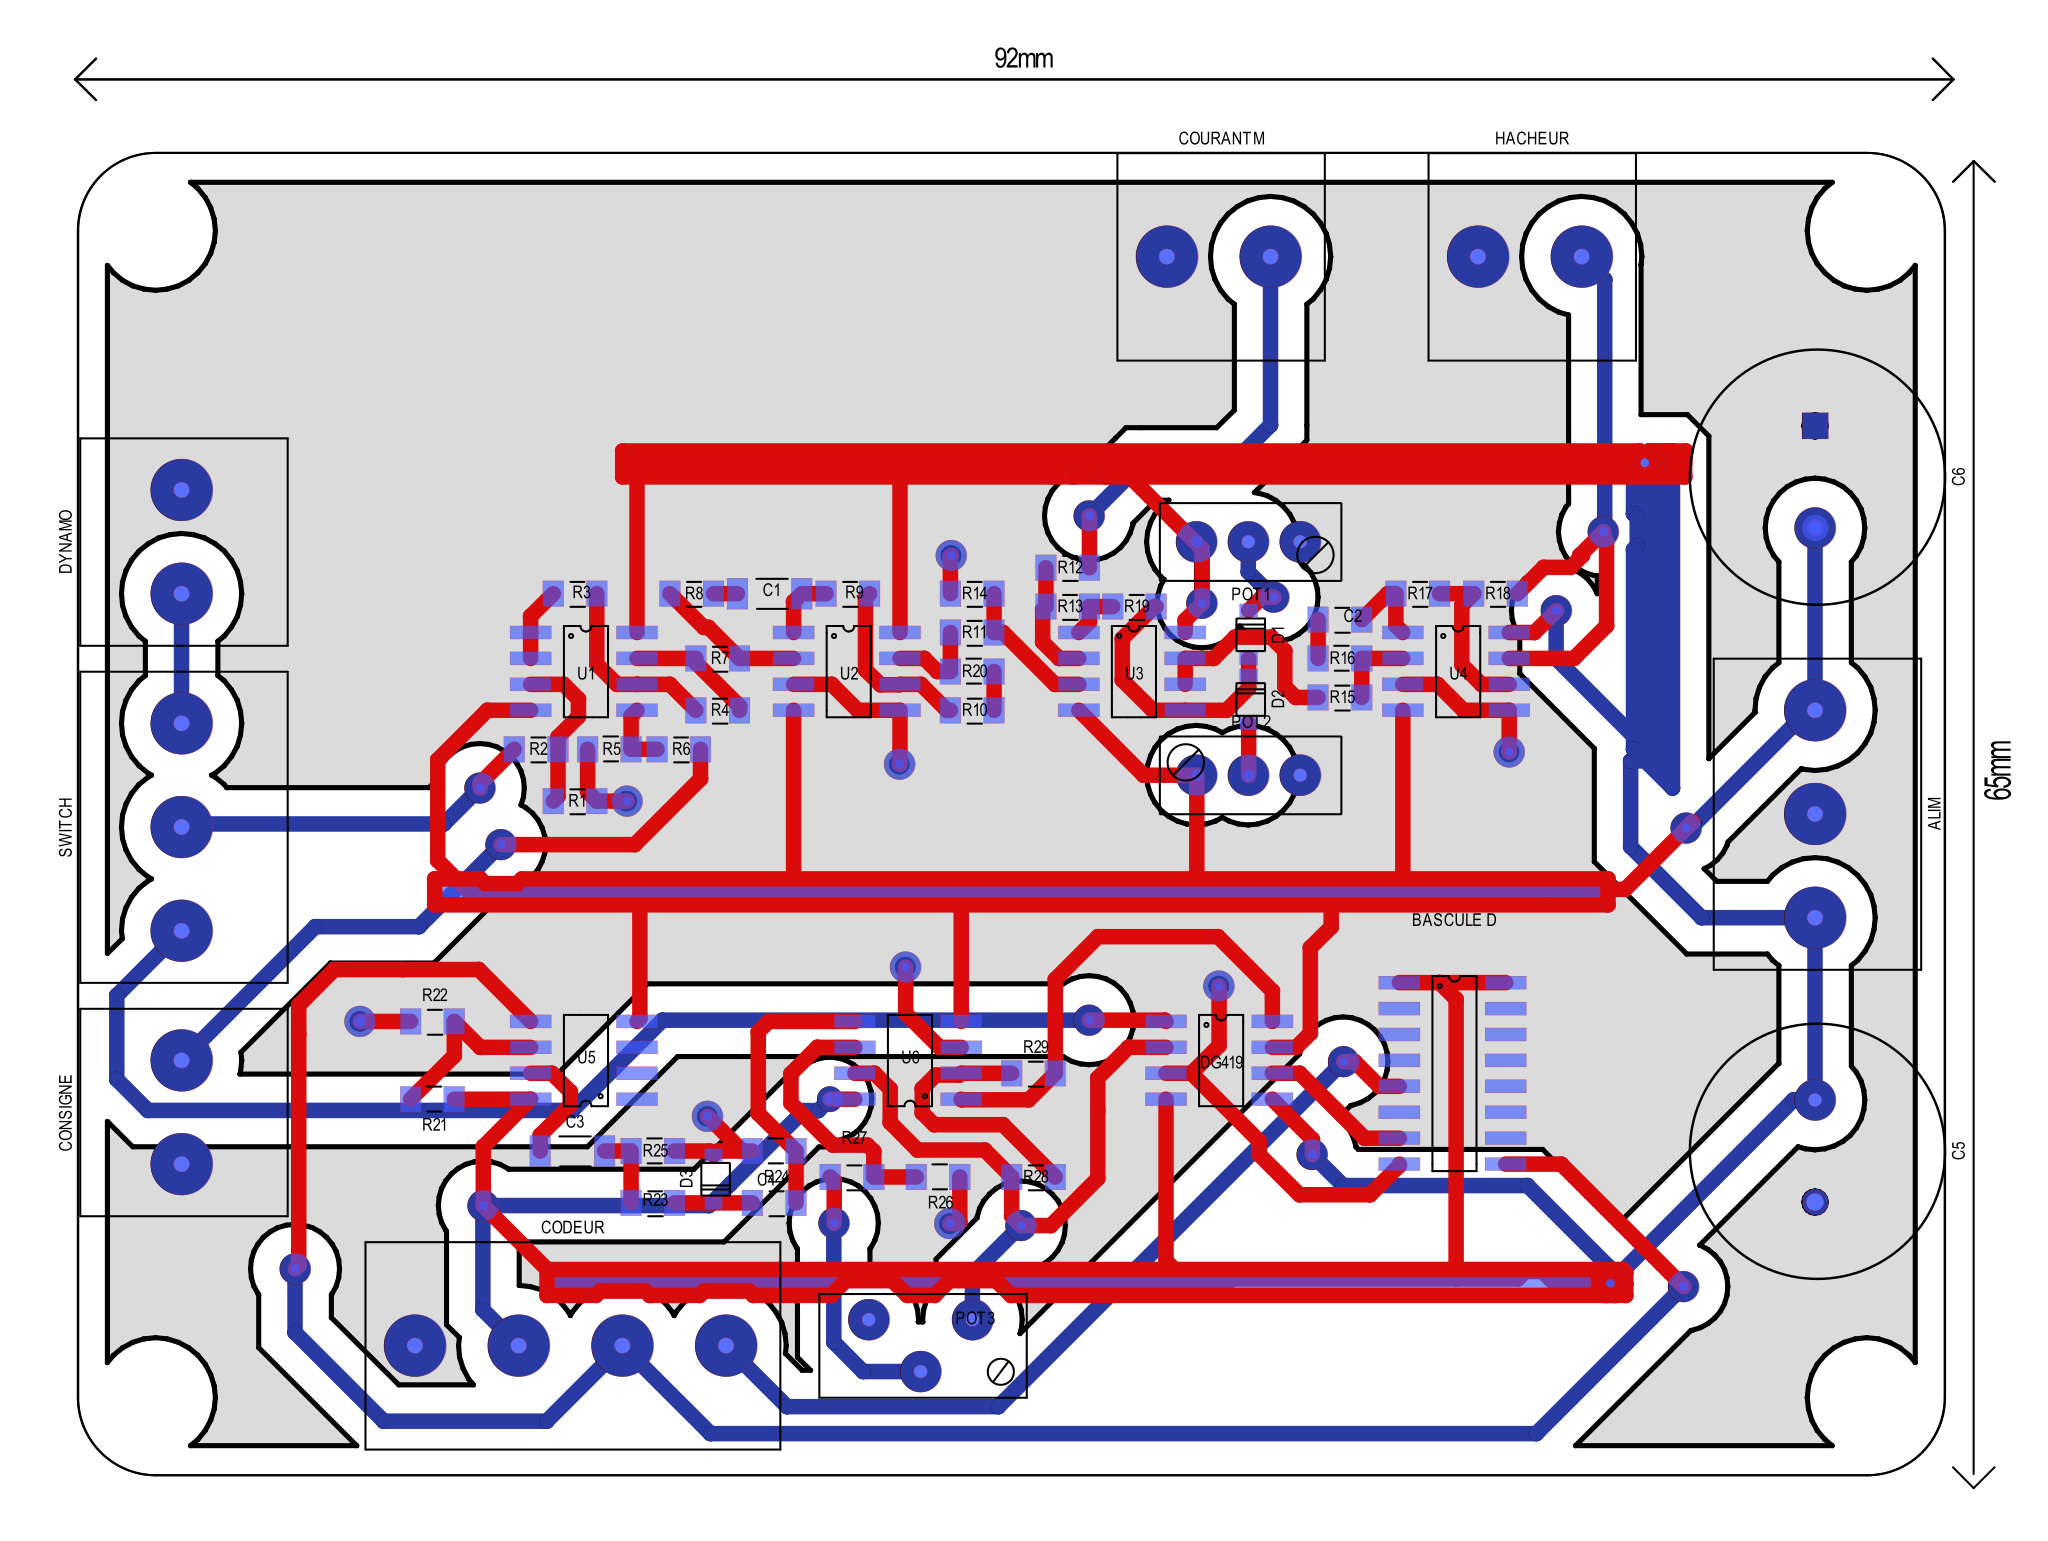
\includegraphics[width=0.8\textwidth]{images/Image PCB/Carte_PCB.pdf}
    \caption{Schéma de la conception du PCB}
    \label{fig:pcb_design}
\end{figure}
\figref{Figure \ref{fig:pcb_design}}{Modélisation\_Finale\_VALIDE\_13\_01\_2026/07\_Conception\_PCB/PCB\_Final\_ProjetGES7\_2025\_27\_11.pdsprj}

Concernant le placement des composants sur le PCB, nous avons répartis les composants sur deux "étages". Le premier étage (celui du haut sur l'image \ref{fig:pcb_design}) comporte toute la chaine d'asservissement du moteur en courant et en vitesse. Tandis que le second étage (celui du bas sur l'image \ref{fig:pcb_design}) contient les composants liés au traitement du signal de sortie du codeur incrémental.


\newpage
En ce qui concerne le connecteur VGA, nous avons également conçu son PCB et son schéma électrique dans \textit{Proteus}, en respectant le standard de câblage VGA prescrit sur Moodle pour assurer une bonne compatibilité avec l'équipement que nous utilisons.

\begin{figure}[H]
    \centering
    \begin{subfigure}[t]{0.48\textwidth}
        \centering
        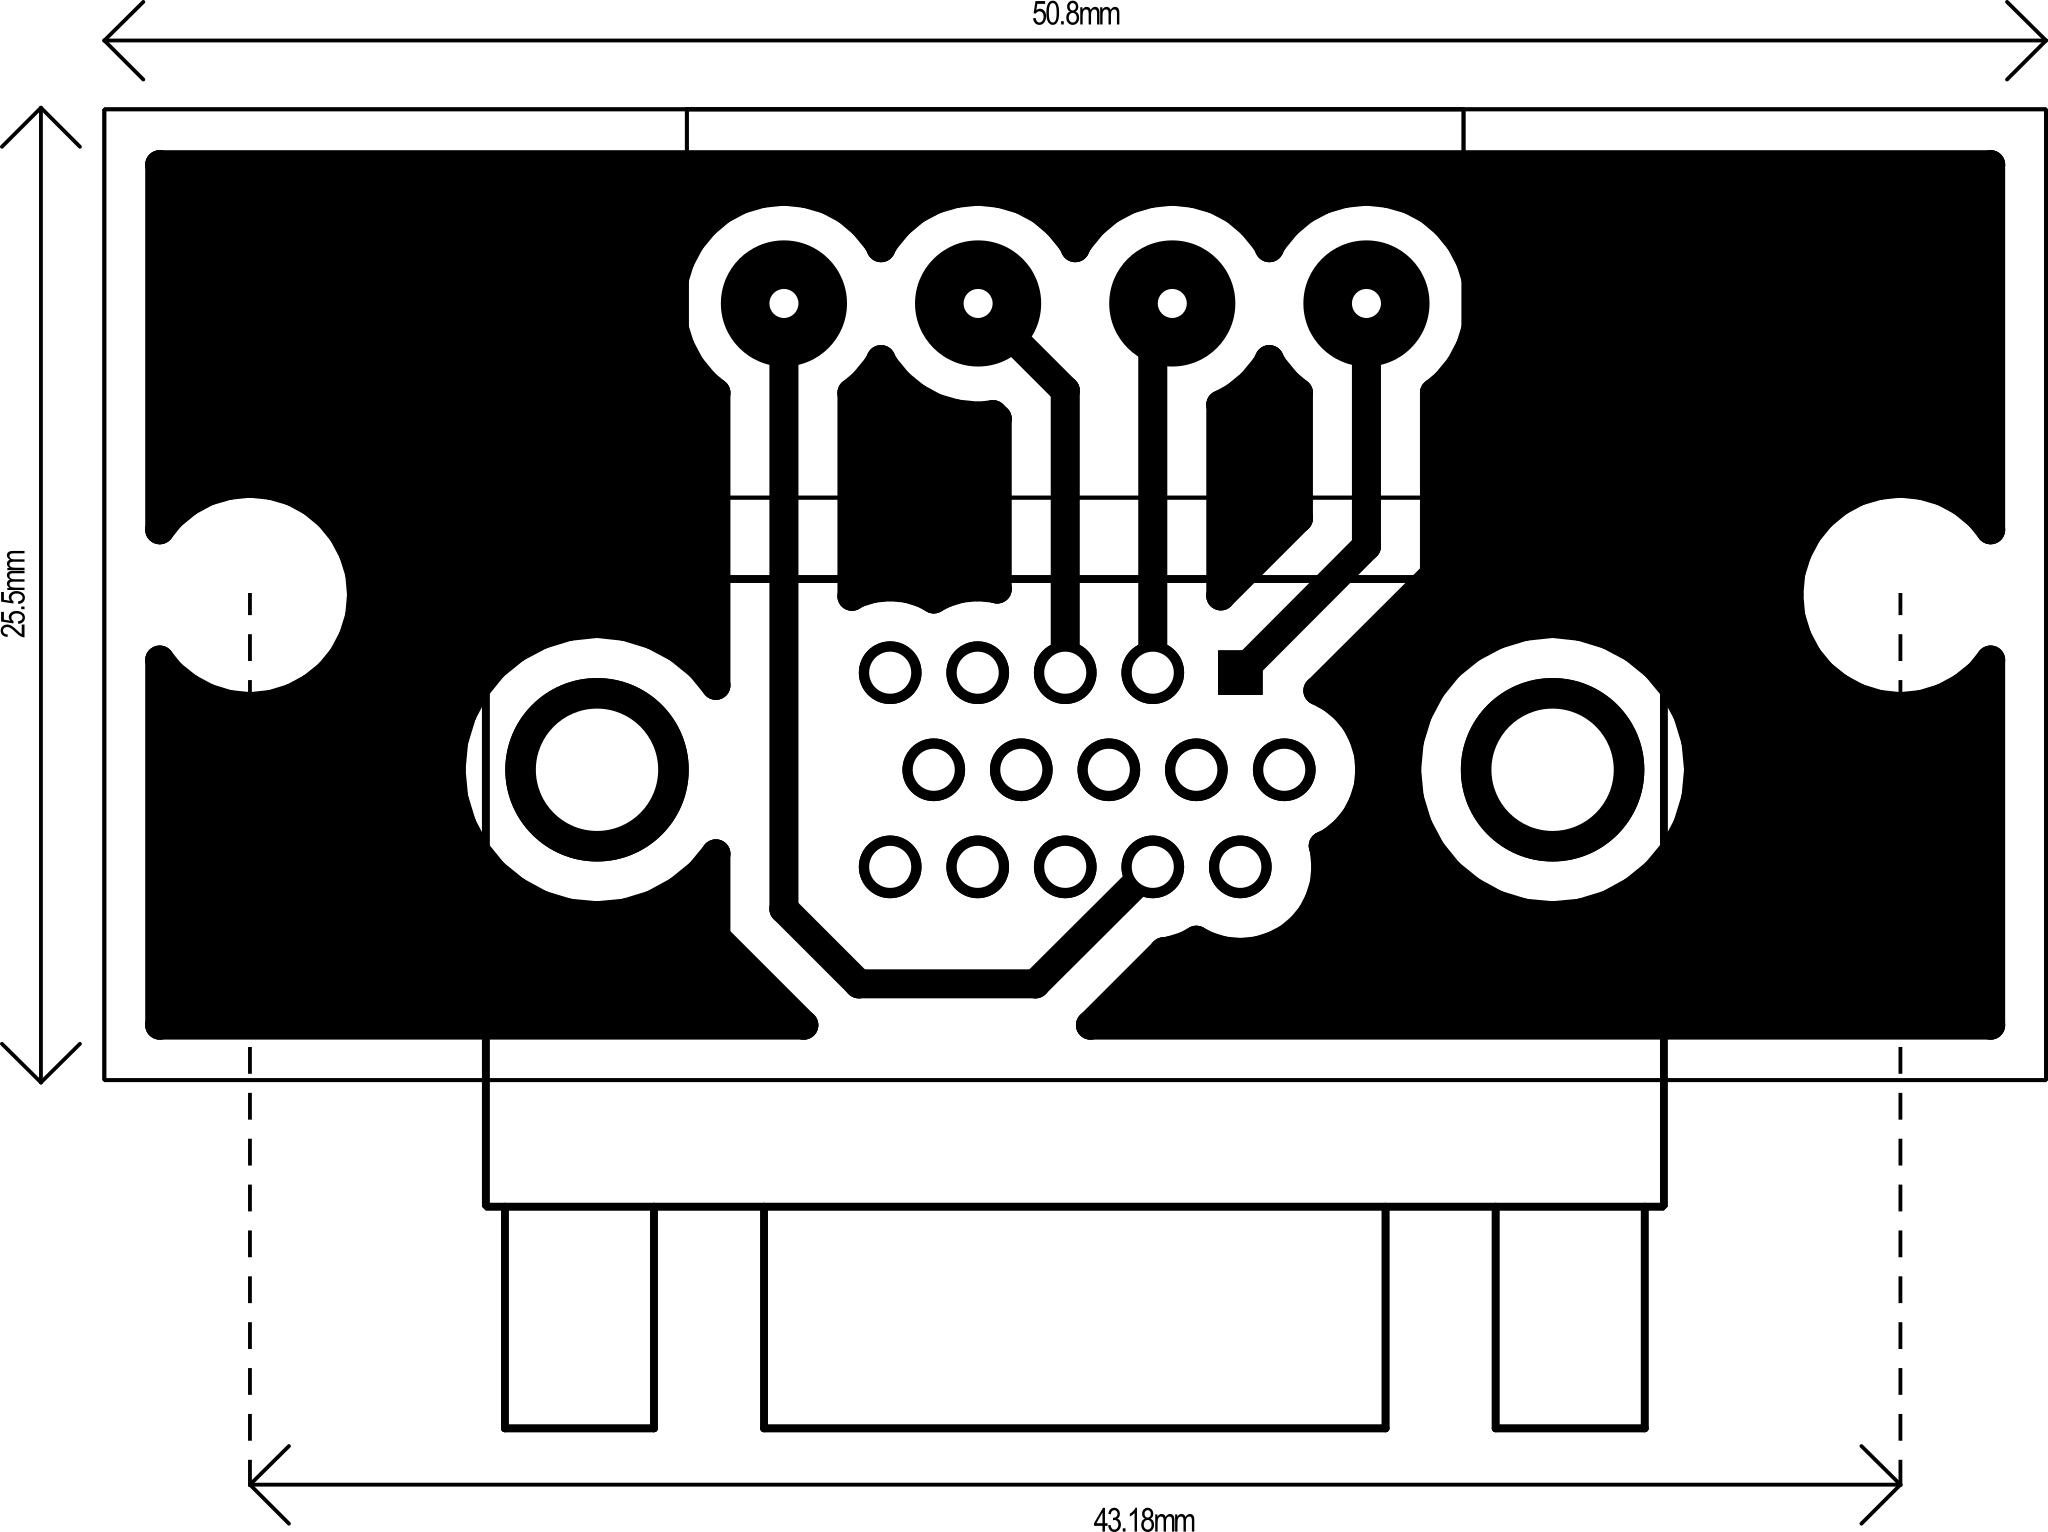
\includegraphics[width=\textwidth]{images/Image PCB/VGA_PCB.pdf}
        \caption{PCB du connecteur VGA}
    \end{subfigure}
    \hfill
    \begin{subfigure}[t]{0.35\textwidth}
        \centering
        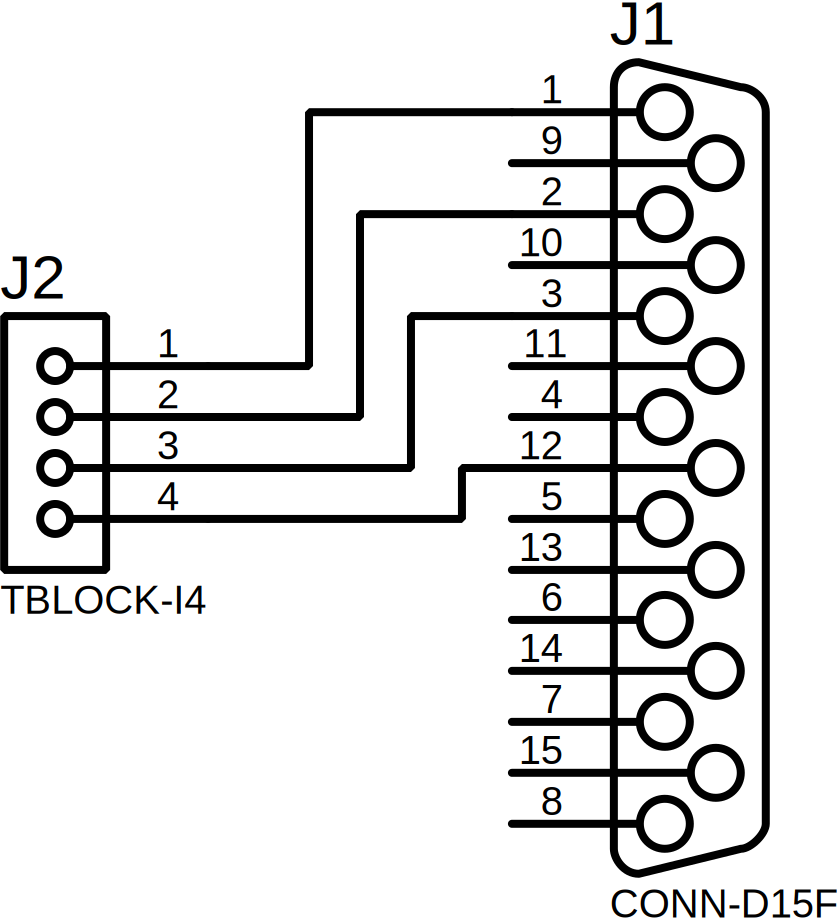
\includegraphics[width=\textwidth]{images/Image PCB/VGA_SCHEMA.pdf}
        \caption{Schéma du connecteur VGA}
    \end{subfigure}
    \caption{Conception du connecteur VGA}
    \label{fig:vga_design}
\end{figure}
\figref{Figure \ref{fig:vga_design}}{Modélisation\_Finale\_VALIDE\_13\_01\_2026/07\_Conception\_PCB/Carte VGA.pdsprj}
\chapter{Assemblage du système}

\section{Commande des composants}

En parallèle de la réalisation du circuit imprimé, nous avons réalisé la commande de composants chez le fournisseur Farnell.

 Le budget étant restreint à 25\,\euro, nous avons fait en sorte de récupérer un maximum de composants déjà présents en PFGE pour limiter le coût de notre commande. De plus, nous avons mutualisé les commandes des différents groupes pour éviter les frais de livraison et diminuer le coût de certains composants achetés en plus gros lots.

Voici la liste des composants que nous avons dû commander :

\begin{tableau}[H]
    \centering
    \begin{tabular}{|l|l|c|c|c|}
        \hline
        \textbf{Composant} & \textbf{Référence} & \textbf{Lien Farnell} & \textbf{Quantité} & \textbf{Prix HT} \\
        \hline
        TL082 & TL082CDT & \href{https://fr.farnell.com/stmicroelectronics/tl082cdt/amplificateur-op-4mhz-0-a-85-c/dp/3367325}{Lien} & 6 & 3,52\,\euro \\
        \hline
        Diodes & 1N4148WS & \href{https://fr.farnell.com/onsemi/1n4148ws/diode-petit-signal-75v-1-5a-sod/dp/2453269}{Lien} & 3 & 0,50\,\euro \\
        \hline
        Potentiomètre 10k$\Omega$ & T93YA103KT20 & \href{https://fr.farnell.com/vishay/t93ya103kt20/potentiometre-trimmer-10k-23-tours/dp/1141404}{Lien} & 2 & 1,90\,\euro \\
        \hline
        Bascule D & HEF40175BT,653 & \href{https://fr.farnell.com/nexperia/hef40175bt-653/bascule-d-40-a-85-c/dp/3442180}{Lien} & 1 & 1,06\,\euro \\
        \hline
        MUX & DG419DY-E3 & \href{https://fr.farnell.com/vishay/dg419dy-e3/ic-mux-precision-cmos-smd/dp/1469446}{Lien} & 1 & 1,57\,\euro \\
        \hline
        Capacité 470 $\mu$F & 25ZLK470M8X20 & \href{https://fr.farnell.com/rubycon/25zlk470m8x20/condensateur-470-f-25v-20/dp/1831286}{Lien} & 2 & 0,83\,\euro \\
        \hline
        Résistance 47k$\Omega$ & CRCW080547K0FKEA & \href{https://fr.farnell.com/vishay/crcw080547k0fkea/res-couche-epaisse-47k-1-0-125w/dp/1469929}{Lien} & 1 & 0,22\,\euro \\
        \hline
        Résistance 8,2k$\Omega$ & MCWF08P8201FTL & \href{https://fr.farnell.com/multicomp-pro/mcwf08p8201ftl/res-couche-epaisse-8-2k-1-0-25w/dp/2694155}{Lien} & 1 & 0,11\,\euro \\
        \hline
        Résistance 560k$\Omega$ & ESR10EZPF5603 & \href{https://fr.farnell.com/rohm/esr10ezpf5603/res-560k-1-0-4w-couche-paisse/dp/4009519}{Lien} & 1 & 0,75\,\euro \\
        \hline
        Capacité 560 nF & MC1206B564K250CT & \href{https://fr.farnell.com/multicomp-pro/mc1206b564k250ct/cond-0-56-f-25v-10-x7r-1206/dp/1759323}{Lien} & 1 & 0,79\,\euro \\
        \hline
        Capacité 6.8 nF & MC1206B682K201CT & \href{https://fr.farnell.com/multicomp-pro/mc1206b682k201ct/cond-6800pf-200v-10-x7r-1206/dp/1855871}{Lien} & 1 & 0,41\,\euro \\
        \hline
        Capacité 1.2 nF & CC1206JKNPOZBN122 & \href{https://fr.farnell.com/yageo/cc1206jknpozbn122/cond-1200pf-630v-mlcc-1206/dp/4166976}{Lien} & 1 & 0,63\,\euro \\
        \hline
        \hline
        \textbf{TOTAL TTC} & & & & \textbf{14,80\,\euro} \\
        \hline
    \end{tabular}
    \caption{Liste des composants commandés}
    \label{tab:composants}
\end{tableau}

\section{Soudure du PCB}

\noindent
\begin{minipage}[t]{0.5\textwidth}
\vspace{0pt}
Une fois que le PCB a été produit par les techniciens et que nous avons reçu la commande, nous sommes passés à la soudure de la carte.

Pour ce faire, nous avions décidé de réaliser une carte entièrement avec des composants montés en surface pour obtenir la carte la plus petite possible. Nous avons donc réalisé en premier la soudure des composants CMS au four à souder, nous avons donc placé les AOP, résistances, capacités et diodes ainsi que la bascule D et l'interrupteur commandé.

Une fois ces composants soudés, nous nous sommes occupés des composants traversant : les différents borniers, potentiomètres et capacités de découplage. Nous avons soudé ces éléments au fer à souder.

Cela nous donne le PCB visible ci-contre.
\end{minipage}
\hfill
\begin{minipage}[t]{0.48\textwidth}
\vspace{-5pt}
\begin{figure}[H]
    \centering
    \includegraphics[width=\textwidth]{images/Image PCB/image3.jpg}
    \caption{PCB après soudure des composants}
    \label{fig:pcb_soudure}
\end{figure}
\end{minipage}

Pour ce qui est de la connexion de notre carte au système réel, nous devons utiliser des câbles coaxiaux pour récupérer les différentes tensions utiles au fonctionnement du système. De plus, notre système doit être alimenté en +15 V et -15 V à l'aide d'une alimentation de laboratoire.

Enfin, il doit être possible de choisir avec quel capteur nous réalisons l'asservissement, donc nous utilisons un interrupteur pour basculer entre la dynamo tachymétrique et le codeur incrémental qui est relié à un port VGA.

Ce qui fait que nous devons réaliser la soudure de fils reliant la carte à ces composants de connectique :
\begin{itemize}
    \item 4 fiches BNC
    \item 3 fiches bananes
    \item 1 interrupteur
    \item 1 connecteur VGA
\end{itemize}



\section{Réalisation du boîtier}

Pour maintenir le PCB et les connectiques en place, nous avons réalisé une boîte imprimée en 3D pour y fixer tous les composants.

Cette boîte a été pensée pour être la plus pratique possible si des modifications doivent être réalisées. C'est pourquoi nous avons décidé de fixer la totalité des composants sous le couvercle de cette boîte pour que, si nous voulons l'ouvrir, nous ayons facilement accès à tous les composants. Le but était d'éviter que des fils relient le couvercle et la boîte, ce qui complique l'ouverture.

Nous avons aussi fait en sorte d'indiquer sur le couvercle l'utilité de chaque connectique en imprimant le texte d'une autre couleur.

\noindent
\begin{minipage}[t]{0.40\textwidth}
\vspace{0pt}
\begin{figure}[H]
    \centering
    \includegraphics[width=\textwidth]{images/Modelisation3d/Vue3D.png}
    \caption{Vue 3D du boîtier}
    \label{fig:boitier_3d}
\end{figure}
\end{minipage}
\hfill
\begin{minipage}[t]{0.55\textwidth}
\vspace{0pt}
\begin{figure}[H]
    \centering
    \includegraphics[width=\textwidth]{images/Modelisation3d/Vue3DOuvert.png}
    \caption{Vue 3D du boîtier ouvert}
    \label{fig:boitier_3d_ouvert}
\end{figure}
\end{minipage}

\vspace{0.5cm}

Nous avons mis en place plusieurs éléments visant à rendre notre boîte plus fonctionnelle :
\begin{itemize}
    \item Des empreintes à double meplat pour fixer les fiches BNC, évitant ainsi qu'elles ne tournent lors des connexions/déconnexions. Cela permet également d'aligner parfaitement les fiches BNC.
    \item Un épaulement sur le pourtour du couvercle pour qu'il s'emboîte parfaitement dans la boîte, même sans être vissé, et ainsi éviter toute entrée de poussière.
    \item Des pieds en caoutchouc pour éviter que la boîte ne glisse sur le poste de travail.
\end{itemize}

\noindent
\begin{minipage}[t]{0.30\textwidth}
\vspace{0pt}
\begin{figure}[H]
    \centering
    \includegraphics[width=\textwidth]{images/Modelisation3d/Meplat.png}
    \caption{Empreintes à double meplat}
    \label{fig:meplat}
\end{figure}
\end{minipage}
\hfill
\begin{minipage}[t]{0.30\textwidth}
\vspace{0pt}
\begin{figure}[H]
    \centering
    \includegraphics[width=\textwidth]{images/Modelisation3d/epaulement.png}
    \caption{Épaulement du couvercle}
    \label{fig:epaulement}
\end{figure}
\end{minipage}
\hfill
\begin{minipage}[t]{0.30\textwidth}
\vspace{0pt}
\begin{figure}[H]
    \centering
    \includegraphics[width=\textwidth]{images/Modelisation3d/Patin.png}
    \caption{Pieds en caoutchouc}
    \label{fig:patin}
\end{figure}
\end{minipage}

\vspace{10pt}

Cette modélisation 3D complète de notre système nous a permis de vérifier que tous les composants rentraient correctement dans la boîte avant de lancer l'impression 3D.

Voici le résultat du projet entièrement assemblé :

\noindent
\begin{minipage}[t]{0.45\textwidth}
\vspace{0pt}
\begin{figure}[H]
    \centering
    \includegraphics[width=\textwidth]{images/Image PCB/image2.jpg}
    \caption{Couvercle du boîtier}
    \label{fig:boitier_couvercle}
\end{figure}
\end{minipage}
\hfill
\begin{minipage}[t]{0.53\textwidth}
\vspace{0pt}
\begin{figure}[H]
    \centering
    \includegraphics[width=\textwidth]{images/Image PCB/image4.jpg}
    \caption{Vue d'ensemble du boîtier}
    \label{fig:boitier_complet}
\end{figure}
\end{minipage}

\vspace{10pt}

Pour réaliser les connexions entre le PCB et les différentes connectiques, nous avons utilisé des câbles que nous avons soudés aux fiches BNC, puis vissés aux borniers du PCB. Les fiches bananes ont été connectées au PCB via des câbles avec des cosses pour effectuer les connexions.
\\
Pour faire cela proprement, nous avons coupé les fils pour qu'ils soient les plus courts possible afin d'éviter leur encombrement. Nous avons également ajouté des gaines thermo-rétractables à chaque soudure pour éviter tout faux contact ou court-circuit.
\\
Voici le PCB relié à tous les organes de connexion :

\begin{figure}[H]
    \centering
    \includegraphics[width=0.8\textwidth]{images/Image PCB/image1.jpg}
    \caption{PCB relié à toutes les connectiques}
    \label{fig:pcb_connectique}
\end{figure}

\chapter{Tests et essais sur la MCC}
\label{chap:essais}

\section{Introduction}

\section{Résolution des problèmes}

\section{Tests et essais finaux}

% --- Conclusion ---
\chapter*{Conclusion}
\addcontentsline{toc}{chapter}{Conclusion}

Ce projet d'asservissement d'une machine à courant continu a permis d'acquérir une vision complète de la chaîne de régulation, depuis la modélisation théorique jusqu'au dimensionnement des composants électroniques réels. À ce stade du projet, il convient de dresser un bilan des travaux réalisés et d'identifier les tâches qui restent à accomplir pour finaliser le système.

\section*{Travaux restant à réaliser}

Malgré les avancées significatives effectuées en simulation et en dimensionnement, plusieurs étapes essentielles restent à compléter avant la finalisation du projet :

\begin{enumerate}
    \item \textbf{Réalisation du circuit imprimé (PCB)} : La conception et la fabrication de la carte électronique permettant d'implémenter physiquement l'ensemble des circuits dimensionnés (correcteurs PI, soustracteurs, limiteur de tension, conditionnement des capteurs).
    
    \item \textbf{Assemblage et câblage du système} : Le montage des composants sur le PCB, le raccordement du moteur, des capteurs (dynamo tachymétrique et codeur incrémental) et de l'alimentation de puissance.
    
    \item \textbf{Tests et validation expérimentale} : La mise en service progressive du système réel, comprenant :
    \begin{itemize}
        \item La vérification du bon fonctionnement des correcteurs PI analogiques
        \item Les tests de l'asservissement en courant puis en vitesse
        \item La comparaison des performances mesurées avec les résultats de simulation
    \end{itemize}
    
    \item \textbf{Réglage et optimisation} : L'ajustement fin des paramètres si nécessaire pour compenser les écarts entre le modèle théorique et la réalité (tolérances des composants, pertes non modélisées, perturbations électromagnétiques).
    
    \item \textbf{Caractérisation complète} : L'évaluation des performances dans différentes conditions de fonctionnement (variations de charge, changements de consigne, robustesse face aux perturbations).
\end{enumerate}

\section*{Bilan et perspectives}

Les travaux menés ont établi des fondations solides pour la réalisation pratique du système. La modélisation mathématique de la MCC a été développée et validée sur MATLAB/Simulink et PSIM, incluant la machine à vide, avec charge mécanique et hacheur quatre quadrants. Deux boucles de régulation en cascade ont été conçues et optimisées, respectant les spécifications du cahier des charges en termes de temps de réponse et de dépassement. L'étude comparative de deux capteurs (dynamo tachymétrique et codeur incrémental) a validé la flexibilité du système, et le dimensionnement complet des circuits analogiques réels a été réalisé avec succès.

\vspace{0.5cm}

Ce projet a permis de développer une méthodologie rigoureuse allant de la modélisation théorique à la réalisation pratique, tout en maîtrisant les outils de simulation et en validant systématiquement chaque étape par comparaison croisée. La réalisation expérimentale du système constituera l'aboutissement de ces travaux, permettant de confronter les prédictions théoriques à la réalité. Les fondations méthodologiques acquises constitueront des atouts précieux pour les développements futurs et l'adaptation du système à d'autres applications industrielles.

\chapter*{Liste des figures et chemins d'accès}
\addcontentsline{toc}{chapter}{Liste des figures et chemins d'accès}

Cette section recense l'ensemble des figures présentes dans ce rapport ainsi que le chemin d'accès aux fichiers de simulation correspondants.

\vspace{0.5cm}

% Cette liste se génère automatiquement à partir des figures ayant un chemin d'accès défini
% via la commande \figpath{label}{chemin} dans le préambule ou les chapitres
{\tiny
\begin{itemize}[leftmargin=0pt, labelwidth=0pt, labelsep=0pt, itemindent=0pt, itemsep=0.3cm]
    \printfigurelist
\end{itemize}
}

\end{document}